\documentclass[a4paper,10pt]{article}\setlength{\textheight}{10in}\setlength{\textwidth}{6.5in}\setlength{\topmargin}{-0.125in}\setlength{\oddsidemargin}{-.2in}\setlength{\evensidemargin}{-.2in}\setlength{\headsep}{0.2in}\setlength{\footskip}{0pt}\usepackage{amsmath}\usepackage{fancyhdr}\usepackage{enumitem}\usepackage{hyperref}\usepackage{xcolor}\usepackage{graphicx}\pagestyle{fancy}
\usepackage{changepage}
\usepackage{makecell}
\usepackage{url}

\lhead{Name: David Mihola}
\chead{M.Number: 12211951}
\rhead{KDDM1 VO (INP.31101UF)}
\fancyfoot{}

\renewcommand\theadfont{\tiny \bfseries}
\renewcommand{\cellalign}{l}

\begin{document}
\begin{enumerate}[topsep=0mm, partopsep=0mm, leftmargin=*]

{\color{blue}
\item\textit{Visual Data Analysis}. Given the dataset ``visual-dataset.csv'' (available in TeachCenter), which comprises a number of features and a binary target feature.
\begin{enumerate}
	\item Provide a number of meaningful visualisations (3-5 visualisations)
	\item Based on the visualisations provide your key interpretation on
	\begin{enumerate}
		\item Are there noteworthy dependencies between the features?
		\item What types of dependency/relationship are there?
		\item Are we expecting the prediction to work well?
	\end{enumerate}
\end{enumerate}
}

First, I have plotted\footnote{\url{https://github.com/xmihol00/kddm1_hws/blob/main/hw1/visualisation.py}} a correlation heat map shown in Figure \ref{fig:heatmap}, to visualise the dependencies between the features. The heat map mostly shows expected dependencies, such as that \textit{total working years} is strongly positively correlated with \textit{age}, \textit{job level} and \textit{monthly income}, that \textit{department} is very strongly positively correlated with \textit{job role} and \textit{education field} or that \textit{job level} has almost perfect positive correlation with \textit{monthly income}. Correlations with the target variable \textit{attrition} are also not surprising, e.g. workers are more likely to leave when they are working a lot of \textit{overtime} or in a certain \textit{job role} and less likely to leave with higher \textit{job level}. Maybe one quite surprising correlation might be the \textit{stock option level} with the \textit{martial status}. I suggest that this might be a coincidence as neither the \textit{stock option level} nor the \textit{martial status} have a strong correlation with any other of the variables. 

Second, based on the visualisations I have made, I can mainly comment on linear and categorical dependencies. There are several positive and negative linear dependencies as described in the paragraph above. Categorical dependencies are also present as already pointed out with the \textit{job role} or the \textit{stock option level}. Some non-linear dependencies might also exist in the data, however they cannot be explored due to the limitations of the used visualization methods.

Third, I am not expecting the prediction to go well, especially when using linear classifiers, as both PCA, see Figure \ref{fig:pca}, and LDA, see Figure \ref{fig:lda}, computed on normalized numerical columns to zero mean and unit variance do not deliver great results. The 3 most linearly correlated features with the target feature, depicted in Figure \ref{fig:top3}, do not also show a clear separation of the features. Another issue, which may arise during prediction, is that there are lot more samples where the target variable has a value of \textit{No}, as shown in Figure \ref{fig:bars}, and that the proportions of the values \textit{Yes} and \textit{No} are similar in all of the bars. Other non-linear classifiers might struggle as well, but this assumption is not based on any non-linear analysis of the dataset. 

%%% Your answer here

{\color{blue}
\newpage\item\textit{Correlation}. Given a dataset, which consists of 1,000 variables (hint: most of them are just random), the goal is to find the relationships between variables, i.e., which and how do the variables relate to each other; what are the dependencies.
The dataset ``correlation-dataset.csv'' can be downloaded from TeachCenter.
\begin{enumerate}
	\item Which methods did you apply to find the relationships, and why?
	\item Which relationships did you find and how do you characterise the relationships (e.g., variable ``Michael'' to ``Christopher'' is linear)?
	\item Which causal relationships between the variables can you find (e.g., variable ``Jessica'' causes ``Matthew'')?
\end{enumerate}
}

I have assumed based on the assignment that the dataset was artificially created and therefore the relationships between the variables might be as well quite artificial. As a result, I have implemented code\footnote{\url{https://github.com/xmihol00/kddm1_hws/blob/main/hw1/visualisation.py}}, which transforms the data using simple functions. The implementation then computes the correlation between all pairs of the original dataset and the transformed dataset, selects the top 10 most correlated pairs excluding correlations of a variable with itself, plots a heat map for visual inspection and saves the largest correlation value for a pair with the used transformation excluding pairs with the absolute value of correlation smaller than 0.5. The 0.5 threshold was selected based on observations, which suggest that a pair of variables is either very correlated or not at all and relatively large absolute values of correlation but still smaller than 0.5 might be just a coincidence. The list of used functions for the transformations is the following: \textit{identity}, \textit{square}, \textit{square root of the absolute value}, \textit{natural logarithm of the absolute value}, \textit{base 10 logarithm of the absolute value}, \textit{exponential}, \textit{reciprocal}, \textit{sine}, \textit{cosine}, \textit{tangent}, \textit{arkus sine of the hyperbolic tangent}, \textit{arkus cosine of the hyperbolic tangent}, \textit{arkus tangent}, \textit{hyperbolic tangent}, \textit{logistic sigmoid}, $2^x$, $x + x^2$, $x + x^2 + x^3$, $x^3$, $x^4$, $x^5$, $x^6$, $x^7$, $x^8$, $x^9$ and $x^{10}$. In some cases, composition with the absolute value or the hyperbolic tangent was necessary to satisfy the domain of the intended function. 

\begin{table}[ht!]
\center
\footnotesize
\begin{tabular}{|l|l|l|r|r|r|r|r|r|}
\hline
\thead{Variable A} & \thead{Variable B} & \thead{Function\\applied\\to\\variable B} & \thead{Pearson\\correlation\\with\\transformed\\variable B} &  \thead{Canonical\\correlation} & \thead{Distance\\correlation} & \thead{Kendall\\rank\\correlation} &  \thead{Maximal\\information\\coefficient} & \thead{Spearman's\\rank\\correlation} \\
\hline
      Anna &      Jakob &                                  $cos(x)$ & -0.976 &            &           &          & 0.898 &  ~    \\[0.15cm]
      Anna & Maximilian &                                  $x^2$ &  0.940 &            &     0.899 &    ~ &       &  ~    \\[0.15cm]
     David &      Felix &                                 $tg(x)$ &  0.597 &      0.596 &     0.563 &    ~ &       & 0.595 \\[0.15cm]
     Elias &       Lena &                        $sigmoid(x)$ &  0.718 &      0.718 &     0.725 &    0.597 &       & 0.777 \\[0.15cm]
      Emma &      Elias &                                  $cos(x)$ &  0.999 &            &           &          & 1.000 &  ~    \\[0.15cm]
      Emma &       Lena &                                  $cos(x)$ &  0.719 &            &           &          & 0.551 &  ~    \\[0.15cm]
     Felix &      David &                        $sigmoid(x)$ &  0.598 &            &           &          & ~ &  ~    \\[0.15cm]
     Jakob &       Anna &                                $identity(x)$ &  0.961 &      0.961 &     0.963 &    0.707 &       & 0.823 \\[0.15cm]
     Jakob & Maximilian &                                 $x ^ 3$ &  0.974 &      0.899 &     0.919 &    0.712 &       & 0.828 \\[0.15cm]
     Jayme &      Laura &                               $x ^{10}$ &  0.871 &            &           &          &       &  ~    \\[0.15cm]
     Laura &      David &                                    $sin(x)$ &  0.836 &            &     0.786 &    0.697 & 0.708 & 0.829 \\[0.15cm]
     Laura &      Felix &                                    $sin(x)$ &  0.501 &            &     ~ &    ~ &       & ~ \\[0.15cm]
      Lena &      Elias &                                 $x ^ 3$ &  0.756 &            &           &          & 0.558 &  ~    \\[0.15cm]
     Marie &       Paul &  $\sqrt{|x|}$ &  0.954 &            &     0.940 &          &       & ~     \\[0.15cm]
Maximilian &       Anna & $log_{10}(|x|)$ &  0.942 &      0.870 &           &          & 0.785 & 0.668 \\[0.15cm]
Maximilian &     Emilia &                      $tanh(x)$ &  0.570 &            &     ~ &    ~ & 0.858 & 0.505 \\[0.15cm]
Maximilian &      Jakob & $ln(|x|)$ &  0.980 &            &           &          & 0.909 & ~     \\[0.15cm]
    Morgan &      Laura &                               $x ^{10}$ &  0.834 &            &           &          &       & ~     \\[0.15cm]
      Paul &      Marie &                             $x + x ^ 2$ &  0.941 &      0.931 &           &    0.775 & 0.905 & 0.934 \\[0.15cm]
\hline
\end{tabular}
\caption{Comparison of correlation (coefficient) between variables using several methods}
\label{tab:corr_transformation_table}
\end{table}

The results using the approach described in the paragraph above are summarized in Table \ref{tab:corr_transformation_table}. I also wanted to test some of the correlation techniques for non-linear data discussed during the lectures. Therefore, I~have implemented all pair correlation also using the \textit{Spearman's rank correlation}, \textit{Kendall rank correlation}, \textit{Canonical correlation}, \textit{Distance correlation} and the \textit{Maximal information coefficient}. While these methods found stronger relationships between the variables in some cases, see the Table \ref{tab:corr_transformation_table}, they do not reveal what kind of relationships are present. However, it is worth noting that using transformations on the other hand can lead to misleading relationships. 

At least I have learnt, that next time it might be better to first use some of the methods for detecting non-linear correlations, plot the highly correlated variables, which I did only as the last step in Figure \ref{fig:best_pairs}, and then either use some of the transformations to further inspect the correlations, or simply estimate the relationships between the variables with a human eye. My estimations with a short discussion are available in Table \ref{tab:my_estimate}.

\begin{table}[ht!]
\center
\begin{tabular}{|l|l|l|}
\hline
\thead{\normalsize Variable A} & \thead{\normalsize Variable B} & \thead{\normalsize My estimate of the relationship} \\
\hline
     Anna &      Jakob & \makecell{The relationship cannot be expressed with a function, closest would be ceil.\\I would call it an overlapping \textit{bucket} relationship, i.e. for increasing Jakob's\\values Anna's values are in buckets with higher floor and ceil. The\\relationship is definitely not cosine, linear would be acceptable.} \\[0.25cm]
     Anna & Maximilian & \makecell{Relationship could be very noisy square, or some kind of very noisy\\exponential, or some kind of a \textit{bucket} relationship.}\\[0.25cm]
     David &      Felix & \makecell{Noisy linear relationship looks as the most likely, probably not tangent nor\\sigmoid}. \\[0.25cm]
     David &      Laura & \makecell{After removing noise and outliers, the correlation would be undefined, as\\Laura's values would be constant (0), or after removing the constant values,\\the relationship could be noisy linear, definitely not sine.} \\[0.25cm]
     Felix & Laura &  \makecell{Same as with David vs Laura, but since any of the method for non-linear\\correlation did not find any strong relationships, it is most likely a false\\positive.} \\[0.25cm]
     Elias & Emma & Almost perfect cosine. \\[0.25cm]
     Elias &  Lena & \makecell{The relationship could be seen as very noisy linear, but rather cannot be\\expressed with a function, I would call it as \textit{triangular} relationship,\\probably not $x^3$.} \\[0.25cm]
     Emilia & Maximilian & \makecell{The relationship cannot be expressed with a single function, but could be\\seen as multiple linear, definitely not hyperbolic tangent.}\\[0.25cm]
     Emma &       Lena & \makecell{An area under squared cosine, not really simple cosine since the relationship\\cannot be expressed with a function.} \\[0.25cm]
     Jakob & Maximilian & \makecell{Something like exponentially increasing \textit{bucket} size relationship, but $x^3$ kind\\of works as well.} \\[0.25cm]
     Jayme &      Laura & \makecell{Same as with David vs Laura, definitely not $x^{10}$ in this case, but since any\\of the method for non-linear correlation did not find strong relationship, it\\is most likely a false positive.} \\[0.25cm] 
     Laura & Morgan & Same as with Jayme vs Laura. \\[0.25cm]
     Marie &       Paul & \makecell{Square root of an absolute value, $x+x^2$ as oppose to square for the reversed\\Paul vs Marie relationship could work as well.} \\[0.25cm]
\hline
\end{tabular}
\caption{My estimate of types of relationships between selected variables (each pair mentioned only once)}
\label{tab:my_estimate}
\end{table}

Although some of the variables are almost perfectly correlated, it does not mean that we can assume causal relationships between them, because, as we were already told multiple times, correlation does not imply causation. Nevertheless, since the dataset is artificially made, I would assume, that some of the variables were directly generated using other variables, but that is just a speculation.

{\color{blue}
\newpage\item \textit{Outliers/Anomalies}. 
\begin{enumerate}
\item For both datasets shown below define yourself, what is the normal behaviour and what are the outliers/anomalies, please indicate in the image the anomalous behaviour
\item Name the algorithms or describe the algorithmic way of how to identify this anomalous behaviour (you may choose different algorithms for each dataset, also describe any necessary preprocessing)
\item Name the assumptions made by your algorithms
\end{enumerate}
\begin{center}
 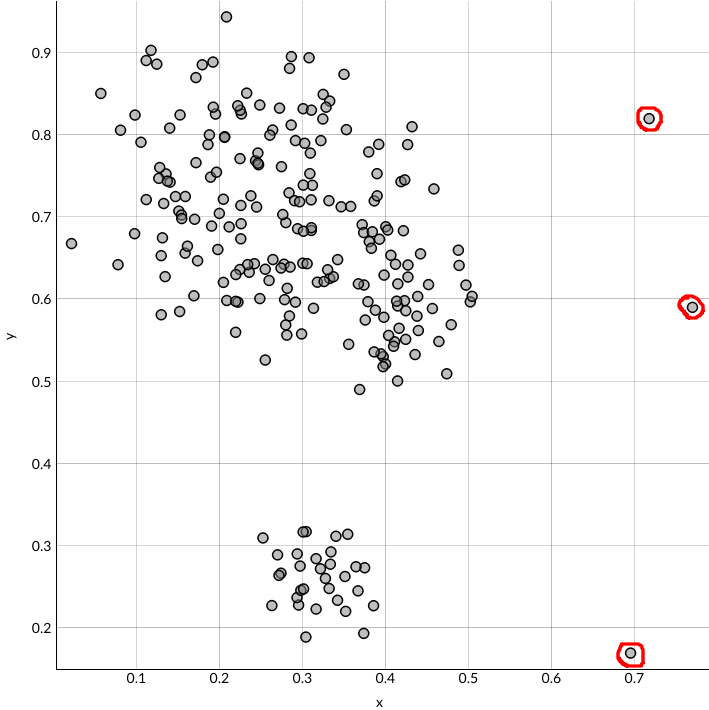
\includegraphics[width=.4\textwidth]{figs/outlier-dataset-1_marked.png}
 \hspace{2cm}
 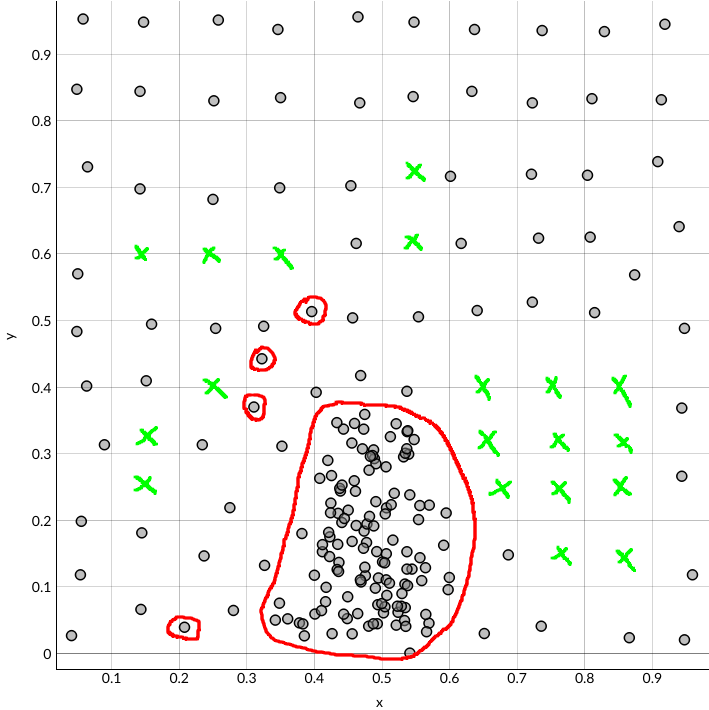
\includegraphics[width=.4\textwidth]{figs/outlier-dataset-2_marked.png}
\end{center}
}

I have marked the samples appearing alone as the outliers and the samples, which have many close neighbours, as the normal behaviour for the first dataset. Clustering the samples and then finding samples far from any of the found clusters could be the best algorithmic way of identifying the outliers. Therefore, I have implemented\footnote{\url{https://github.com/xmihol00/kddm1_hws/blob/main/hw1/cluster_outliers.py}} 3 solutions how to cluster the data and then find outliers without knowing anything about the dataset, i.e. completely unsupervised. The methods are: 
\begin{itemize}
    \item K-means clustering with an Euclidean distance measure for outlier detection, with a threshold equal to 3 times the standard deviations of the distances to the nearest cluster center,
    \item Gaussian mixture models (GMM) clustering with a Mahalanobis distance for outlier detection with a threshold equal to 99 percentiles of the distances to the nearest cluster center,
    \item DBSCAN clustering with default scikit learn parameters.
\end{itemize}
The dataset was normalized to zero mean and unit variance as a preprocessing step. The optimal number of clusters for K-means and GMM clustering was estimated using the silhouette score. Comparison of how each of the methods behaved on an artificially created dataset can be seen in Figure \ref{fig:outliers}. I would personally, also not knowing the ground truth, say that the GMM clustering performed the best. But the results strongly depends on the chosen hyper-parameters, i.e. the threshold, which should be chosen based on the expectations over the dataset, e.g. 1 \% of samples are expected to be outliers. The first two methods assume that outliers are far from the centres of the clusters, the third method assumes that outliers are in low-density regions, i.e. regions with small numbers of samples relative to other regions.

Defining what are the outliers and anomalous behaviour for the second dataset was not that straight forward. Finally, I have decided to mark (red) mainly the sample at the bottom center of the plot as anomalies, i.e. samples that were created by a different process or that are from a different distribution than the unmarked samples. Additionally, I have marked some areas (green), where a sample is expected, as outliers, in this case meant with a reversed understanding to the normal understanding of an outlier, which should be a sample at a far edge of a given distribution, while the marked areas are rather well within the distribution/pattern but with missing samples. I am interpreting the dataset as that the anomaly was caused e.g. by some faulty sensor or by an accidental mix up of two datasets and the so defined outliers might be e.g. caused by interrupts in internet connection. I have not implemented any specific algorithm for this dataset, but my approach to deal with the laid out task would be the following:
\begin{enumerate}
    \item detect the smallest and largest X and Y coordinates, crop the space of interest and normalize it if need, e.g. between 0 and 1, as a preprocessing step,
    \item define the occurring pattern and its hyper-parameters, in this case a grid with a call edge length of 0.1 units and 1 sample per grid cell, the pattern and hyper-parameters could be learned as well,
    \item try to align the grid or any other pattern to the available data samples,
    \item run an algorithm, which traverses the space of interest cell by cell, and for each cell marks samples to be removed or as missing,
    \item increase the robustness of the algorithm e.g. by assessing multiple neighboring cells at once and interpolating occurrences of samples between them. 
\end{enumerate}
The algorithm assumes that there is a well defined pattern in the data.

{\color{blue}
\newpage\item\textit{Missing Values}. The dataset ``missing-values-dataset.csv'' (available on TeachCenter) contains a number of missing values.
\begin{enumerate}
	\item Try to reconstruct why the missing values are missing? What could be an explanation?
	\item What methods do you apply?
	\item What strategies are applicable for the features to deal with the missing values?
	\item For each feature provide an estimate of the arithmetic mean (of the version of the dataset without missing values)?
\end{enumerate}
}

First, I have plotted\footnote{\url{https://github.com/xmihol00/kddm1_hws/blob/main/hw1/missing_values.py}} a correlation heat map of all the columns and histograms of all columns with missing values to find an explanation why the values might be missing. I wanted to inspect the dependencies between the columns with the correlation heat map, while  I was looking for specific ranges of missing values with the histograms, which would suggest a NMAR type of missing values, e.g. that there would be a sudden drop in the number of people reporting English skills smaller than 70. This was not the case for any of the columns, all columns more or less followed the expected distribution based on my assumptions about the human population. Only the histogram for column \textit{height} shown in Figure \ref{fig:height_dis}, was in my opinion very right leaning. The expected histogram would capture two overlapping normal distributions, one for the height of women and second for the height of men, but the overlap is very moderate around 155 cm if any. This can be partially explained by the proportion of samples of men and women in the dataset, but still the average world-wide height is 159 and 171 cm\footnote{\url{https://ourworldindata.org/human-height}} for women and men respectively, which the data do not follow (age is not a factor, since all samples record an age of 20 or higher, location, where the data were collected, could be a factor, but is unknown). Based on this discovery, I have plotted histograms in Figure \ref{fig:gender_dis} of gender, gender when height is missing and gender when books per year are missing. The last based on the assumption that men read less. The figure shows, that men do not report height more often than woman, which with the missing mass in the histogram suggests that there might be a NMAR type of missing values after all, i.e. men might not be reporting their height when it is to small. Missingness in column \textit{books per year} seems unrelated to the gender of the respondents. Next, I~have tried to find similar relationship between age and semester or English skills in Figure \ref{fig:age_distrib}. The figure quite clearly shows, that missing values in the \textit{semester} column depend on the age, i.e. MAR type of missing values -- older people are not studying anymore, whereas missing values in \textit{English skills} column do not depend on it. Lastly, I could not find any other relationships explaining the missing values in columns \textit{likes ananas on pizza}, \textit{English skills} and \textit{books per year}. Therefore, I have concluded that missing values in these columns are of the MCAR type. 

The methods applied for inspection of the missing values, as described in the paragraph above, include correlation, i.e. finding dependencies, data distribution analysis with the use of histograms and common knowledge about the domain of the dataset.

\begin{table}[ht!]
    \centering
    \begin{tabular}{|l|c|l|}
        \hline
        \thead{\normalsize column} & \thead{\normalsize imputed value} & \thead{\normalsize discussion} \\
        \hline
        semester & median (10) & \makecell{The mean (10.977) could be used as well, but I have chosen\\median to keep the integer data type as e.g. 10.977 semesters\\might not be an acceptable value in some use cases.} \\[0.15cm]
        height & \makecell{159 for women,\\171 for men} & \makecell{Based on my assumption made above that the data are biased\\I have chosen the world-wide averages to compensate for it.} \\[0.15cm]
        likes\_ananas\_on\_pizza & 0.5 & \makecell{Both the mean (0.515) and the median (0.554) do not reflect\\well the distribution of the data (most values are close to 0 or\\1), therefore, I have introduced a constant of 0.5 marking an\\undecided state.}\\[0.15cm]
        english\_skills & mean (98.611) & \makecell{I do not have any assumptions about this column, so I have\\rather chosen the mean over the median (98.973) as it will not\\affect the mean in later on computations.}  \\[0.15cm]
        books\_per\_year & mode (2) & \makecell{Although it is not a categorical column, I have still decided to\\impute the missing values with the mode rather than the\\median (3), which would be applicable as well, or the mean\\(3.673), which could also be applicable if the integer data type\\does not have to be kept. The reason is the data distribution,\\which shows that 2 books per year is almost twice as frequent\\than any other of the recorded values.}\\
        \hline
    \end{tabular}
    \caption{Selected values for imputation with a reasoning behind their selection}
    \label{tab:imputation}
\end{table}

The values selected for imputation and the strategies of selecting them are summarized in Table \ref{tab:imputation}.

The estimates of an arithmetic mean for applicable columns of the dataset with imputed missing values are available in Table \ref{tab:mean_estimate}.

\begin{table}[ht!]
    \centering
    \begin{tabular}{|c|c|c|}
        \hline
        \thead{\normalsize column} & \thead{\small \small arithmetic\\\small mean\\\small estimate\\\small rounded\\\small to\\\small 3 decimal\\\small places} & \thead{\normalsize discussion} \\
        \hline
        id & ----- & \makecell{The column is a unique categorical identifier, not a feature,\\computing the arithmetic mean does not make sense.} \\[0.15cm]
        semester & 10.934 & ~ \\[0.15cm]
        gender & ----- & \makecell{The column is purely categorical, computing arithmetic mean does\\not make sense, what a mean gender 0.311 represents? What rather\\makes sense to compute in this case is the percentage of women\\(31 \%) and men (69 \%) in the dataset, assuming that woman is 1\\and man is 0 based on the correlation between height and gender.}\\[0.15cm]
        height & 172.129 & \\[0.15cm]
        age & 25.687 &\\[0.15cm]
        likes\_chocolate & 0.809 & \makecell{The column rather looks like a categorical, but in this case we can\\assume that there can exist some fuzziness in liking and disliking\\chocolate similarly to the perception of ananas on pizza and\\estimating mean in this case makes sense.} \\[0.15cm]
        likes\_ananas\_on\_pizza & 0.511 & \\[0.15cm]
        english\_skills & 98.611 & \\[0.15cm]
        books\_per\_year & 3.602 & \\
        \hline
    \end{tabular}
    \caption{Estimates of an arithmetic mean or an explanation why the estimate should not be made}
    \label{tab:mean_estimate}
\end{table}

\end{enumerate}

\newpage

\begin{figure}
\begin{adjustwidth}{-0.87cm}{}
    \centering
    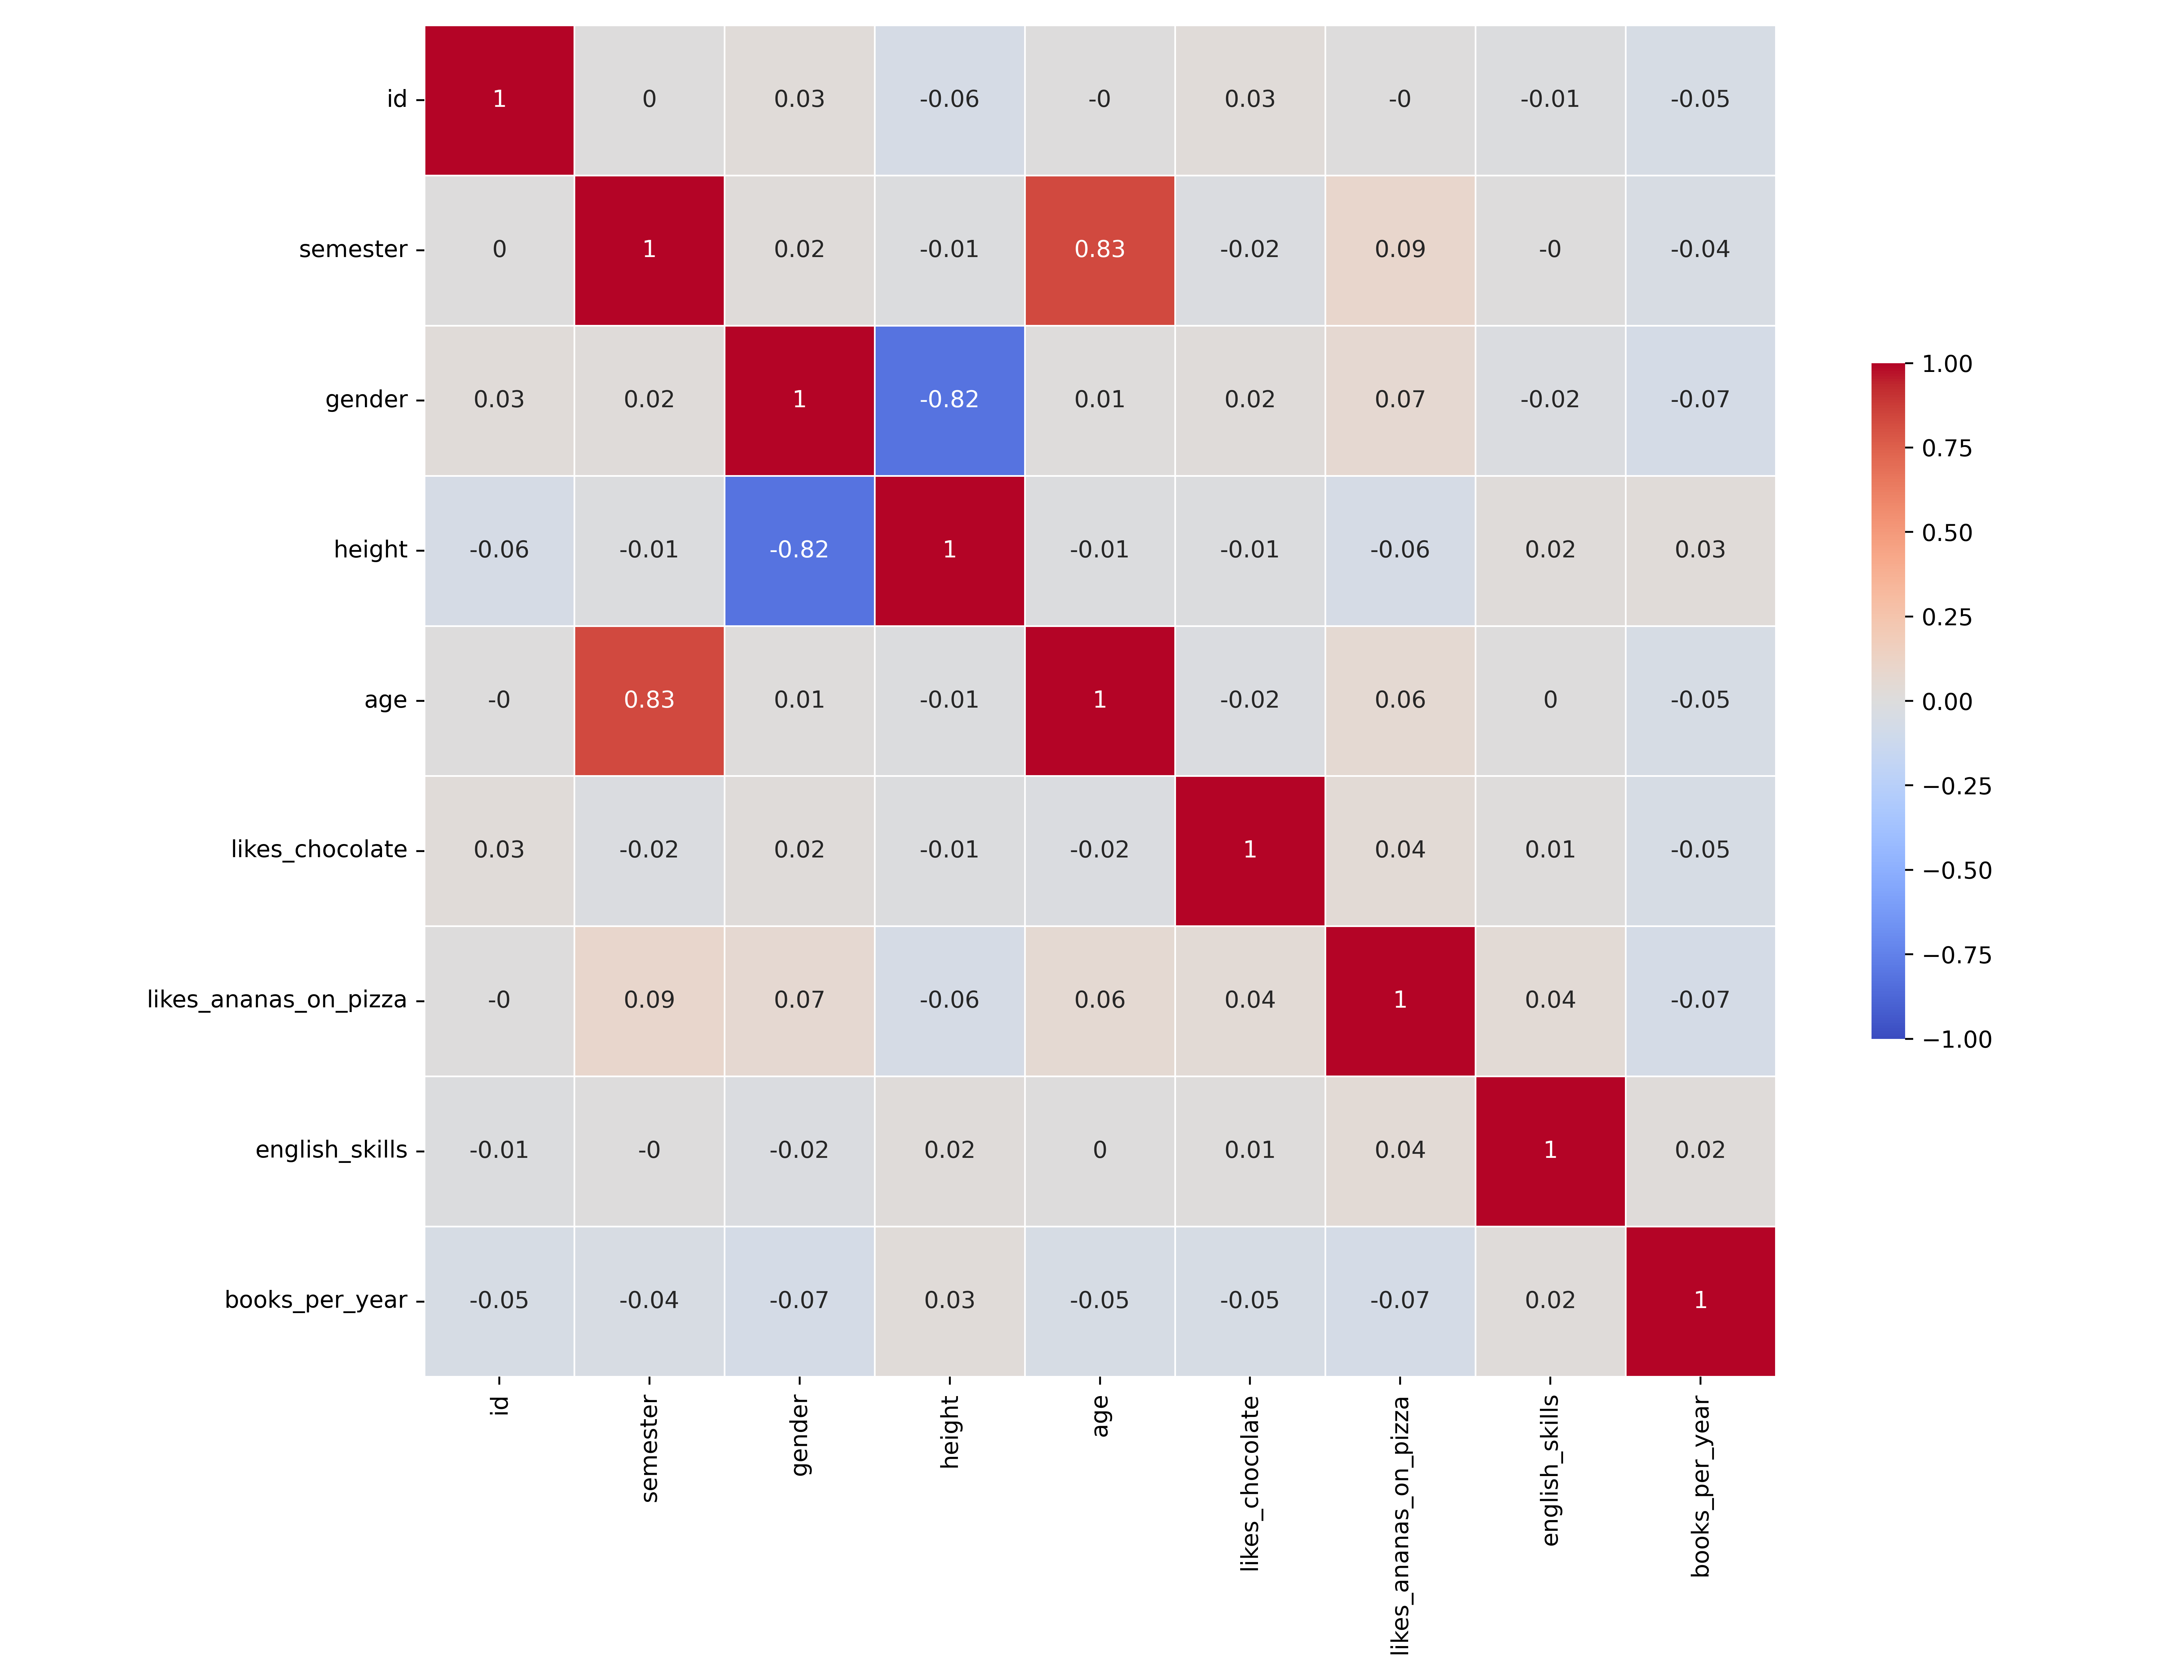
\includegraphics[width=1.22 \textwidth]{figs/correlation_heatmap.png}
    \caption{Task 1 -- correlation heat map}
    \label{fig:heatmap}
\end{adjustwidth}
\end{figure}

\begin{figure}
\begin{adjustwidth}{-0.87cm}{}
    \centering
    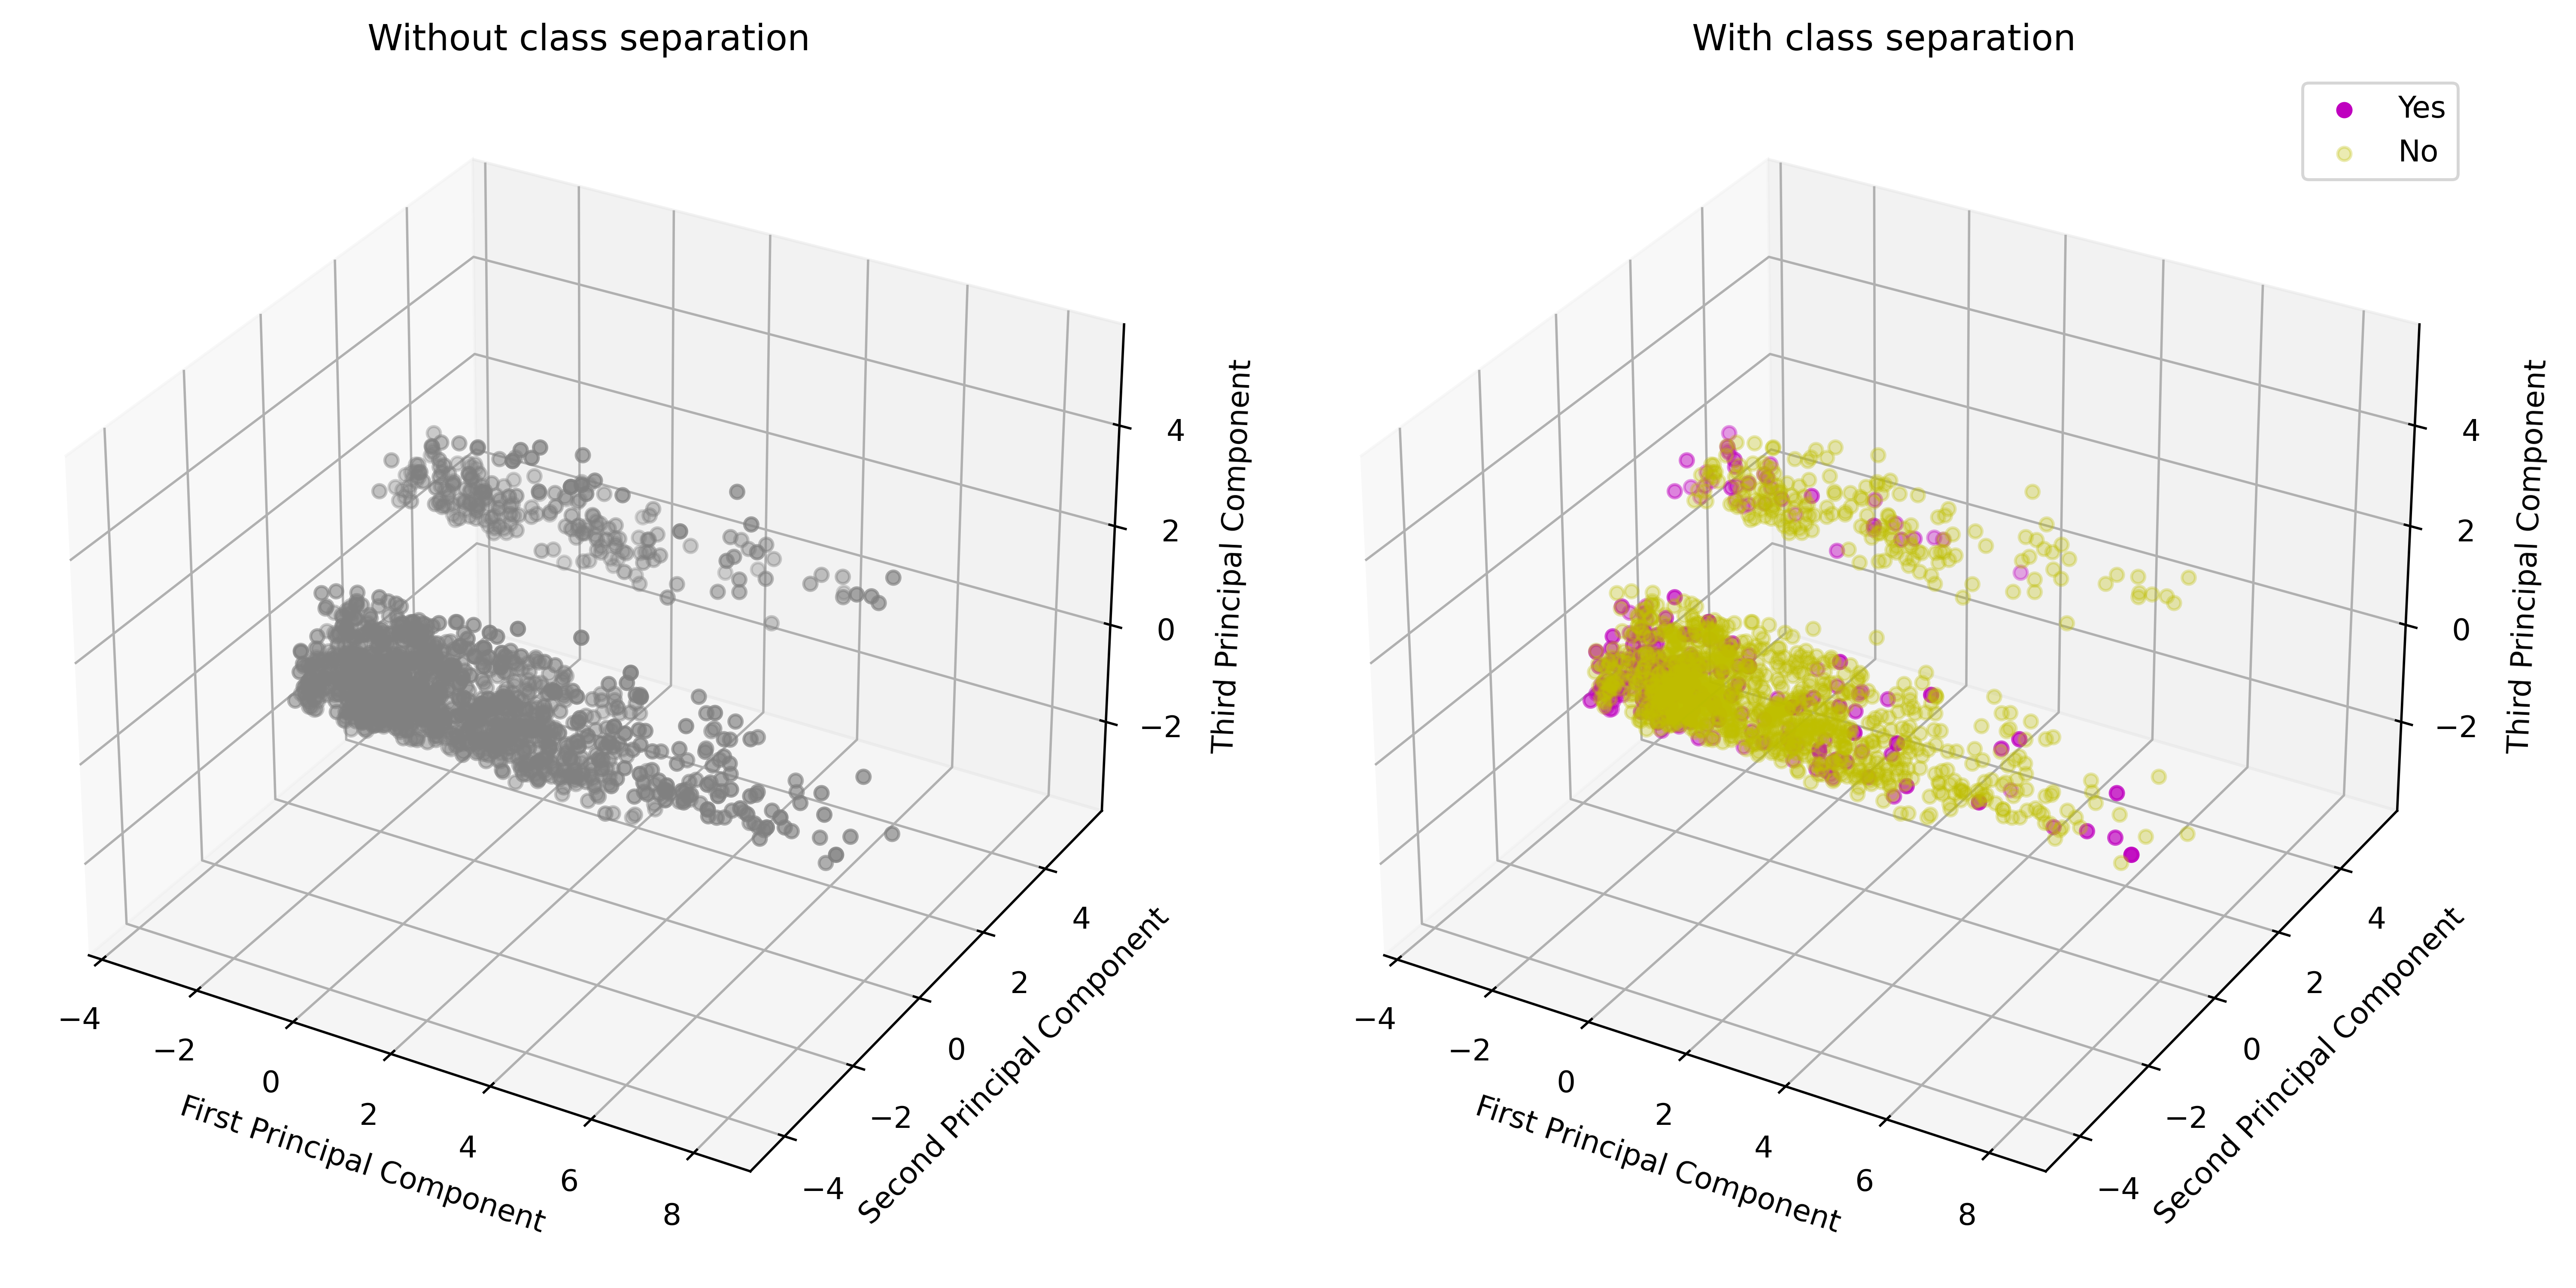
\includegraphics[width=1.1 \textwidth]{figs/pca_3D_subplots.png}
    \caption{Task 1 -- scatter plot of the 3 most significant principal components}
    \label{fig:pca}
\end{adjustwidth}
\end{figure}

\begin{figure}
\begin{adjustwidth}{-0.87cm}{}
    \centering
    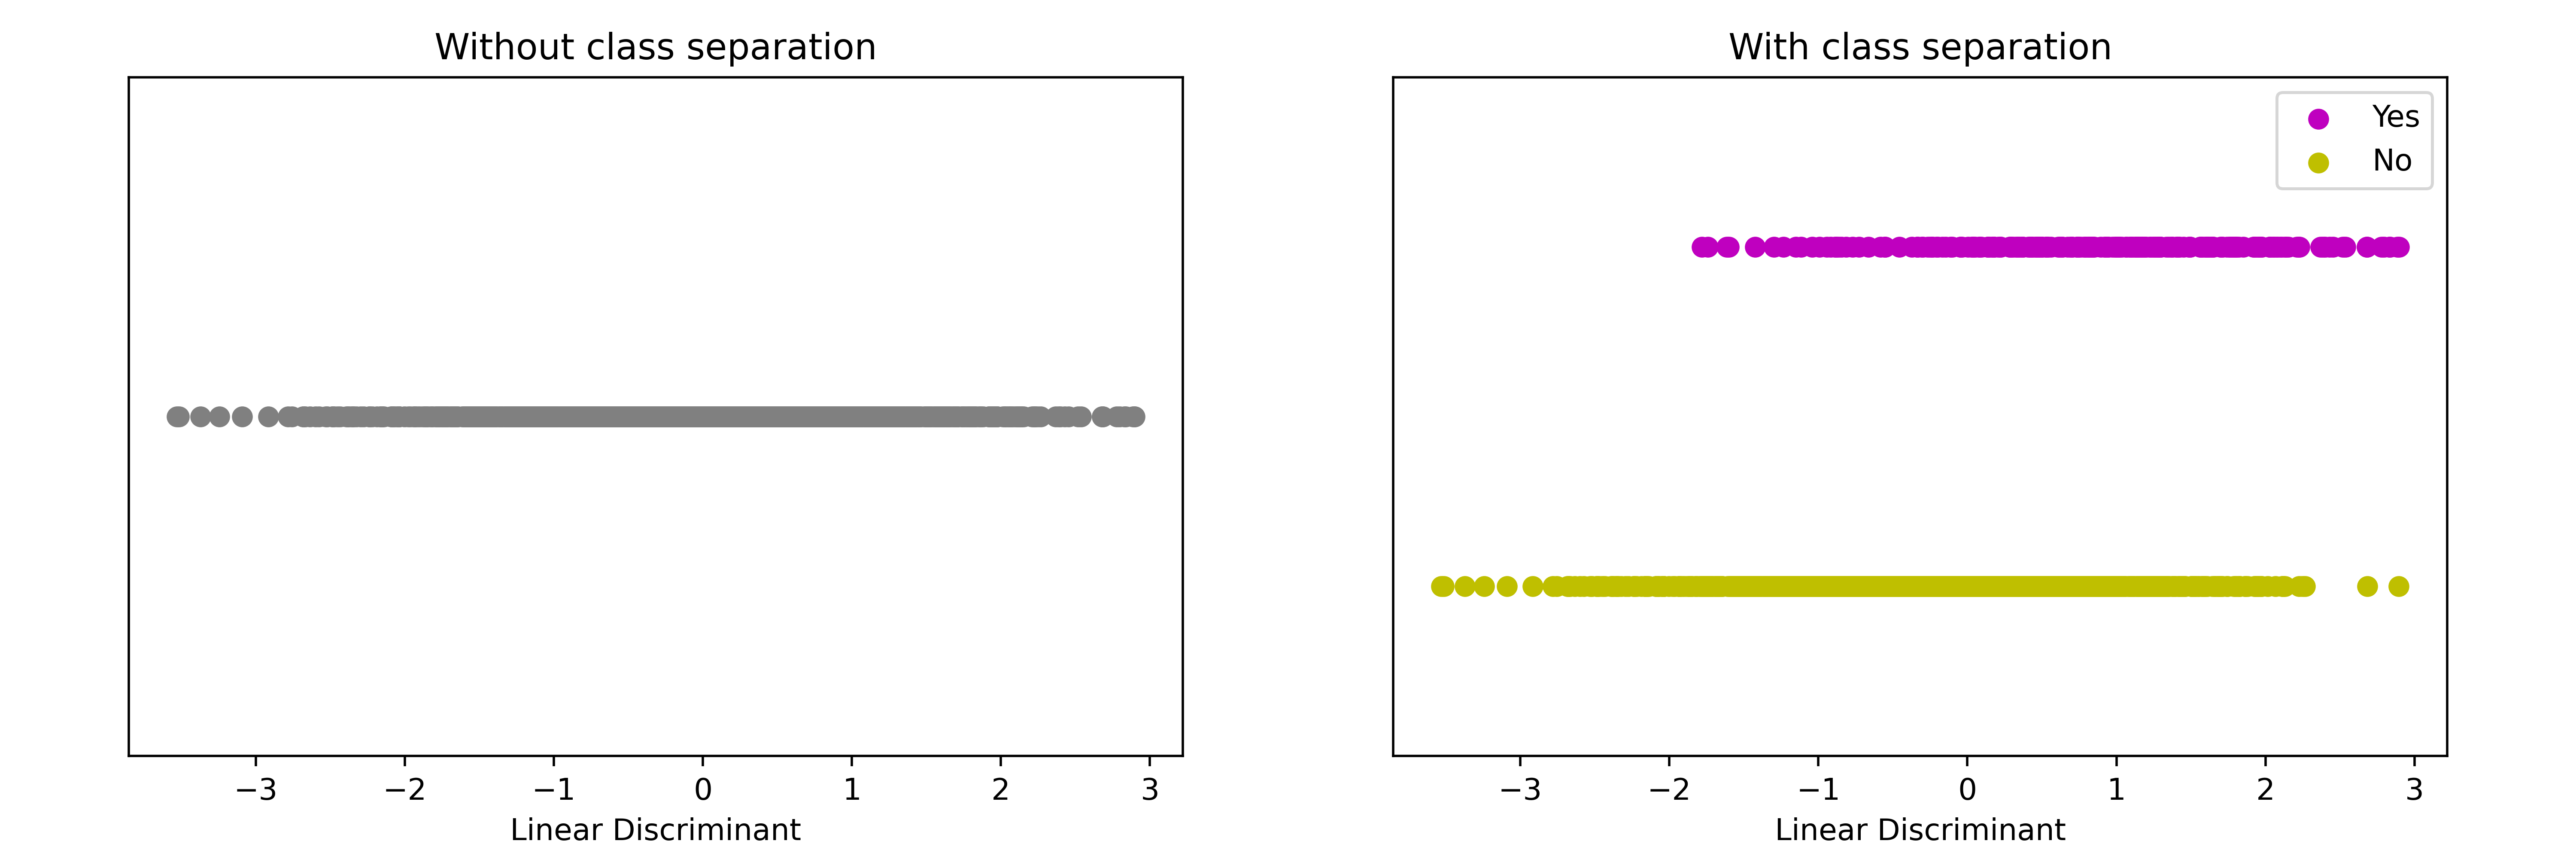
\includegraphics[width=1.1 \textwidth]{figs/lda_1D_subplots.png}
    \caption{Task 1 -- scatter plot of the linear discriminant}
    \label{fig:lda}
\end{adjustwidth}
\end{figure}

\begin{figure}
\begin{adjustwidth}{-0.87cm}{}
    \centering
    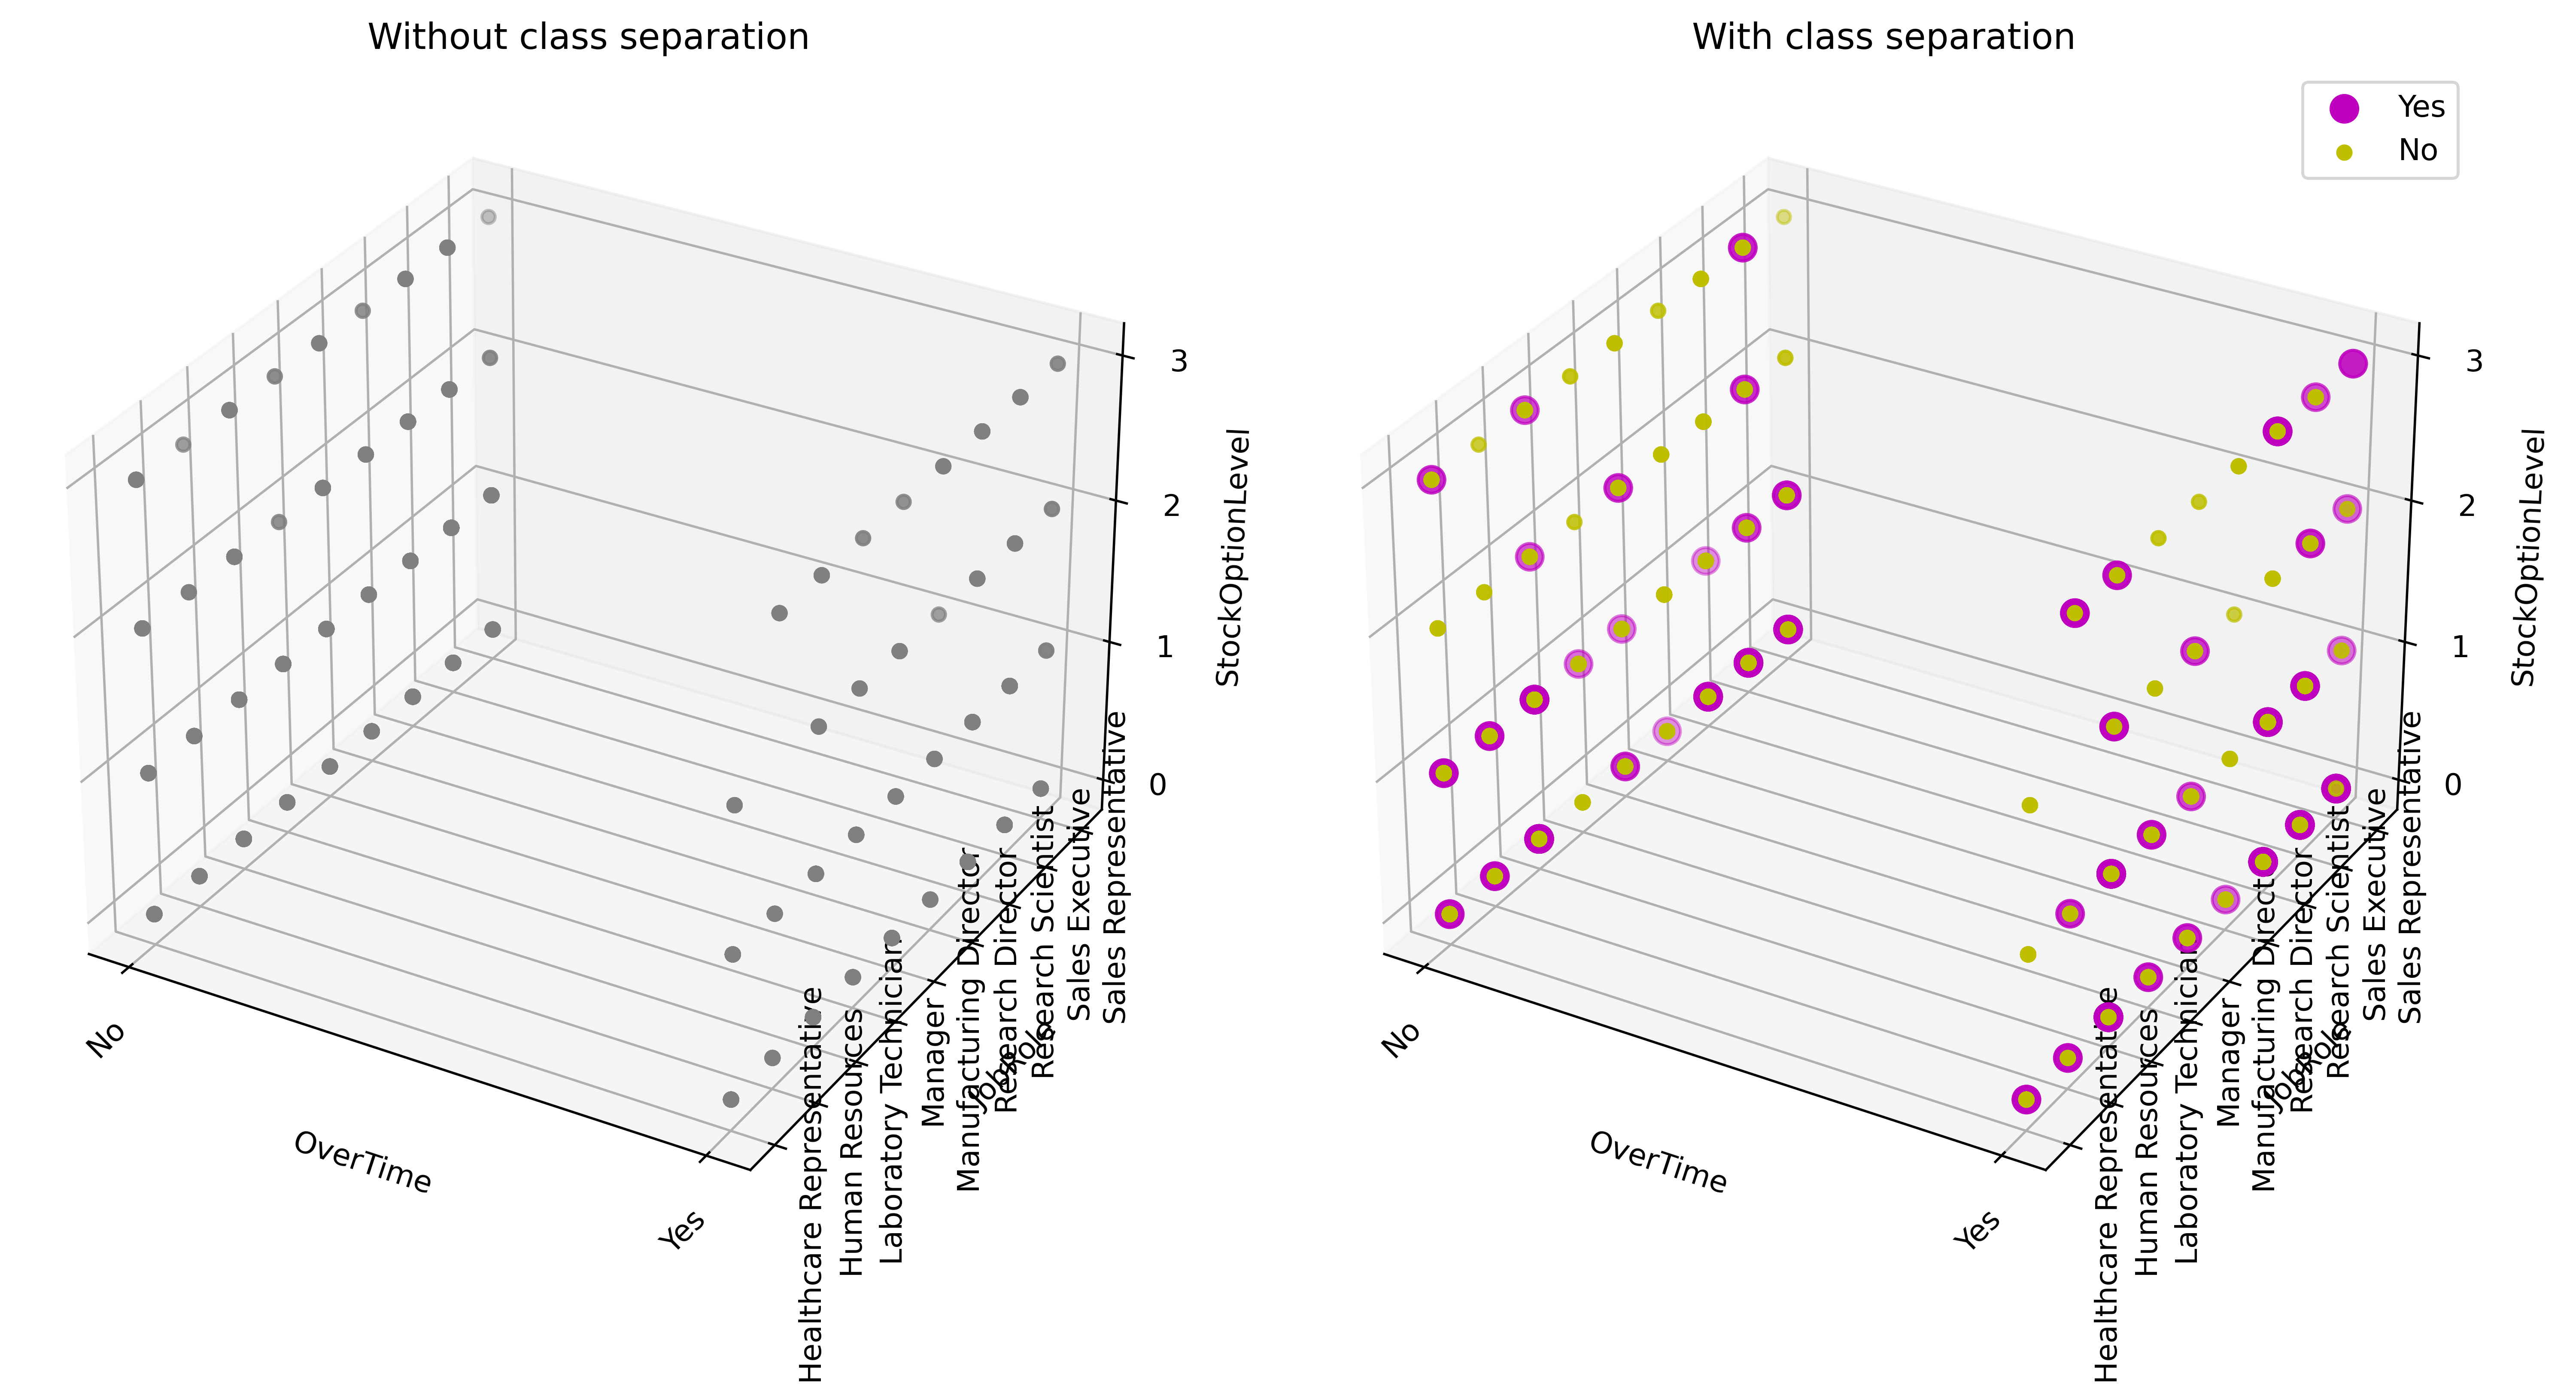
\includegraphics[width=1.1 \textwidth]{figs/feature_importance_3D_subplots.png}
    \caption{Task 1 -- scatter plot of the top 3 most correlated features with the target feature}
    \label{fig:top3}
\end{adjustwidth}
\end{figure}

\begin{figure}
\begin{adjustwidth}{-0.87cm}{-0.2 cm}
    \centering
    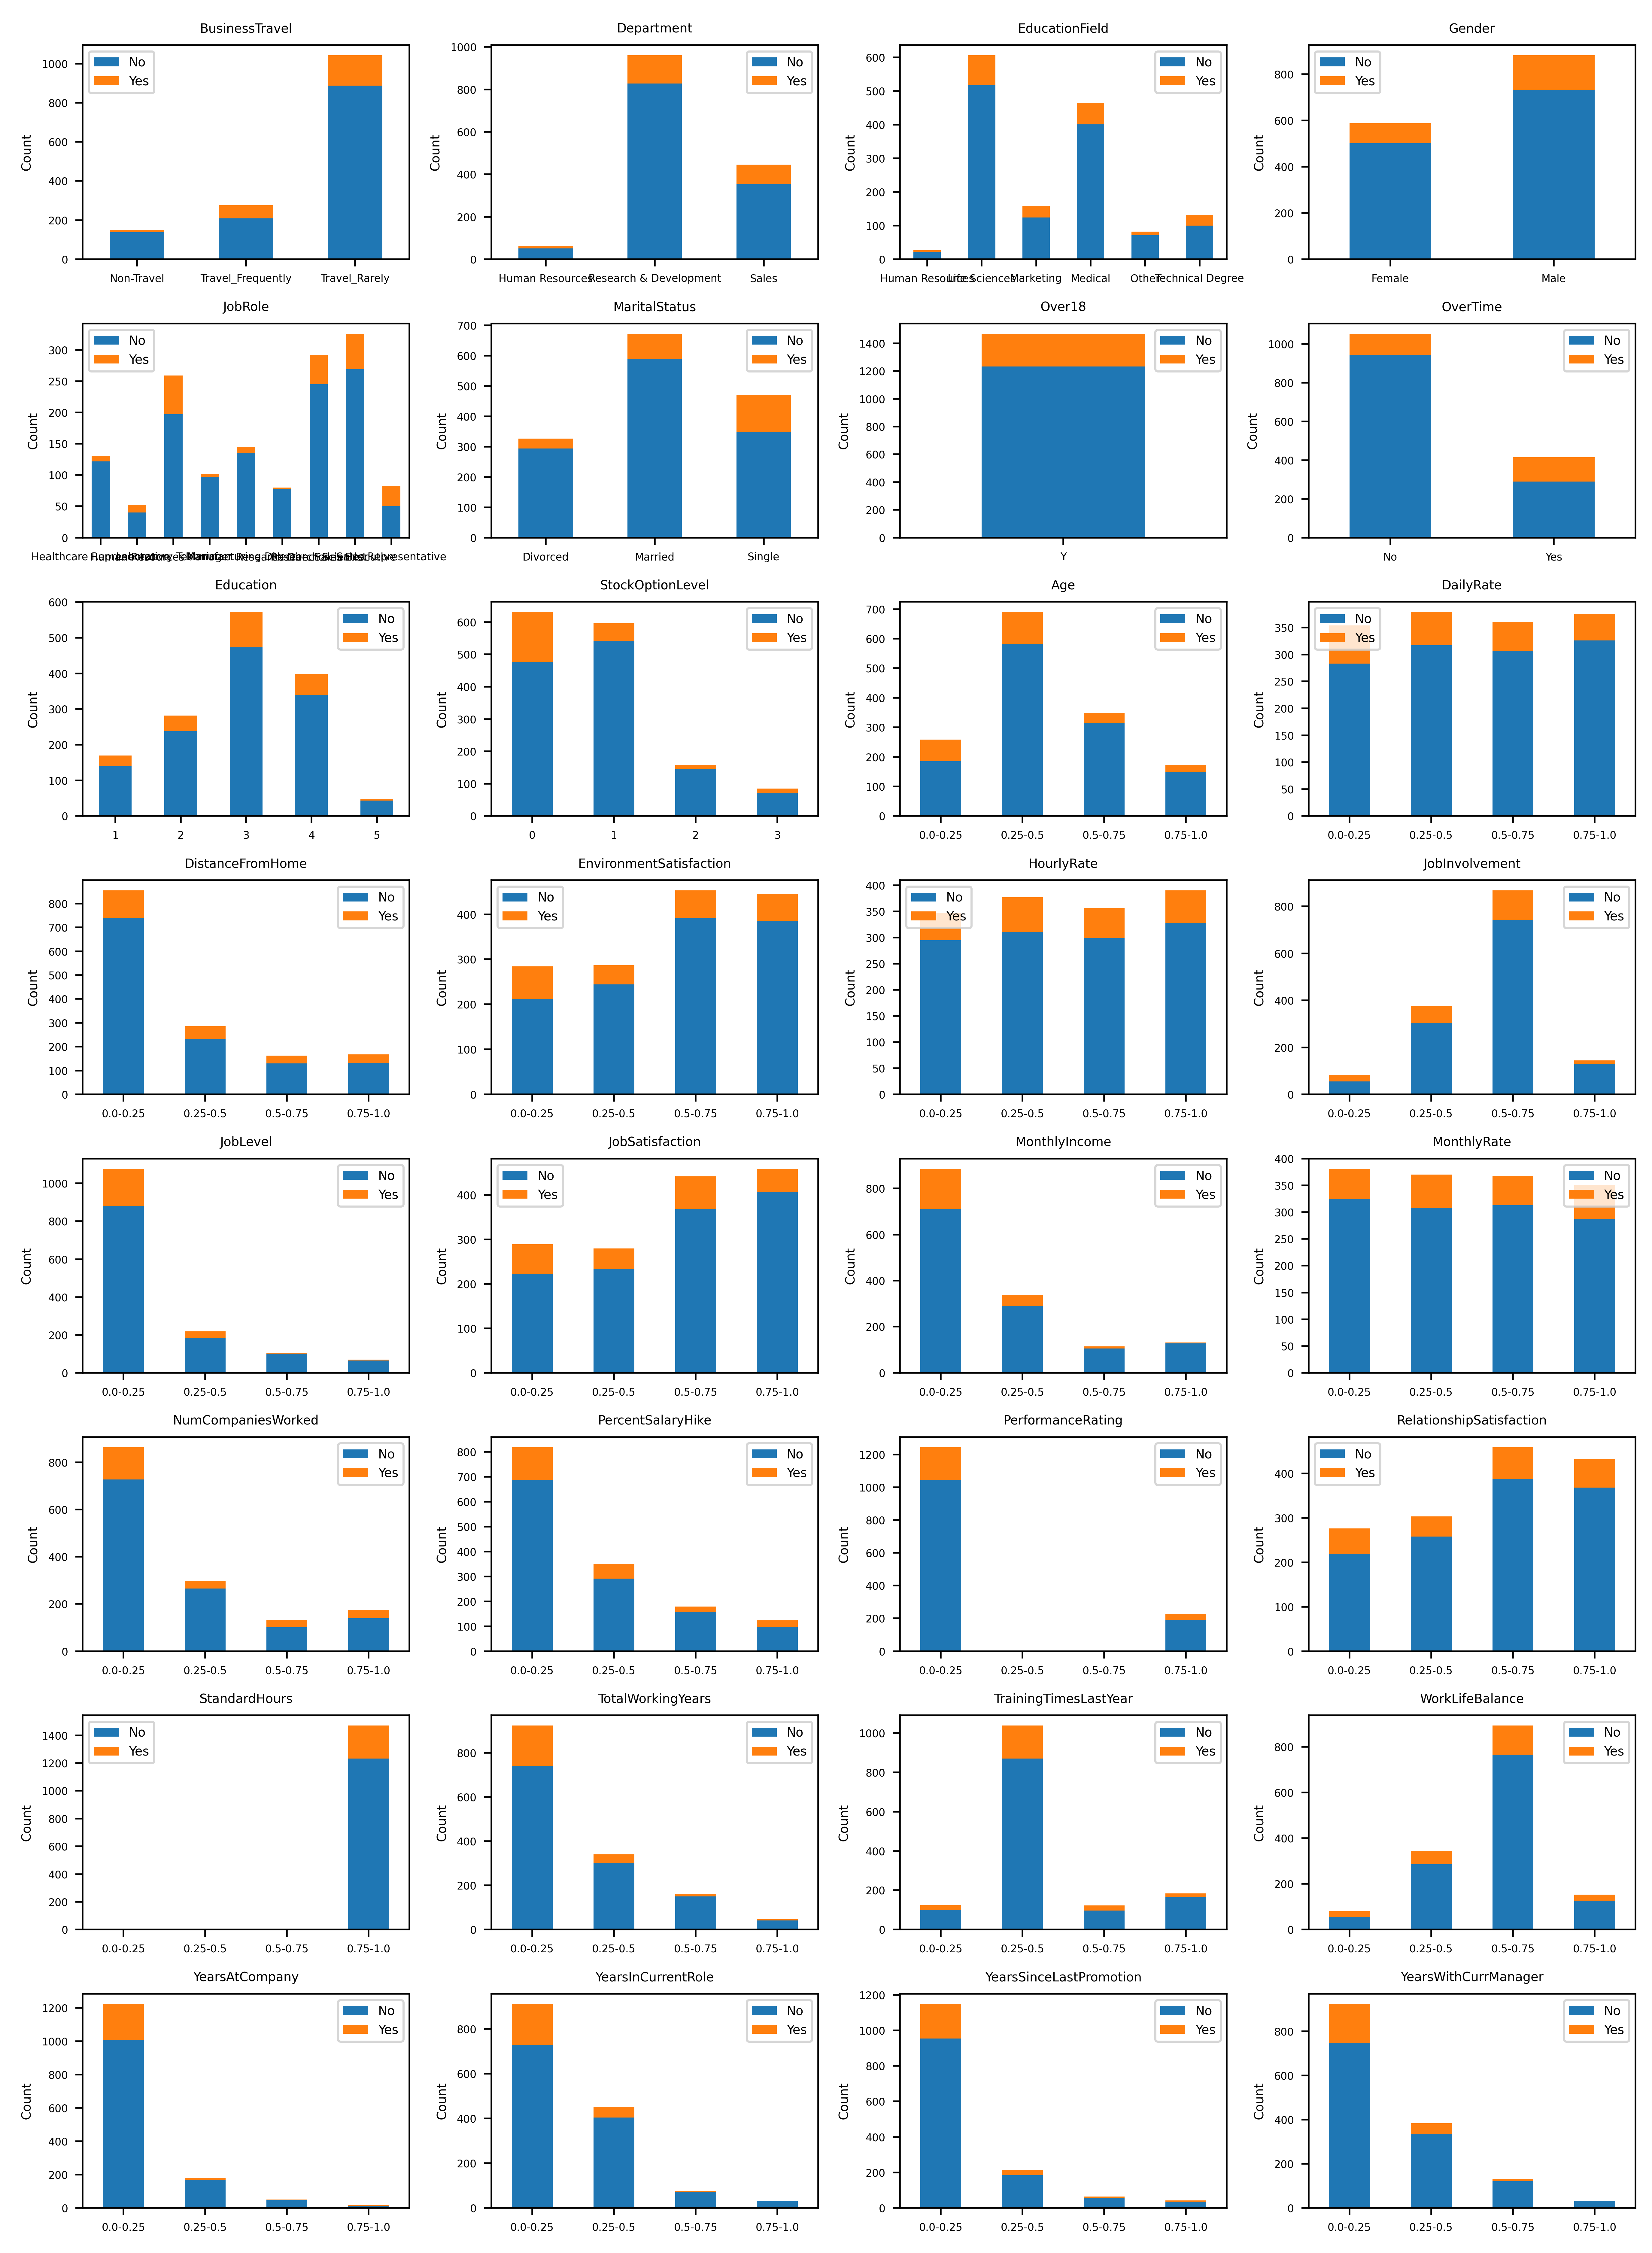
\includegraphics[width=1.1 \textwidth]{figs/bar_plots.png}
    \caption{Task 1 -- bar plots capturing dependencies of the target feature on all of the other features (continuous features are normalized to an interval between 0 and 1 and split to 4 bins)}
    \label{fig:bars}
\end{adjustwidth}
\end{figure}

\begin{figure}
\begin{adjustwidth}{-0.87cm}{}
    \centering
    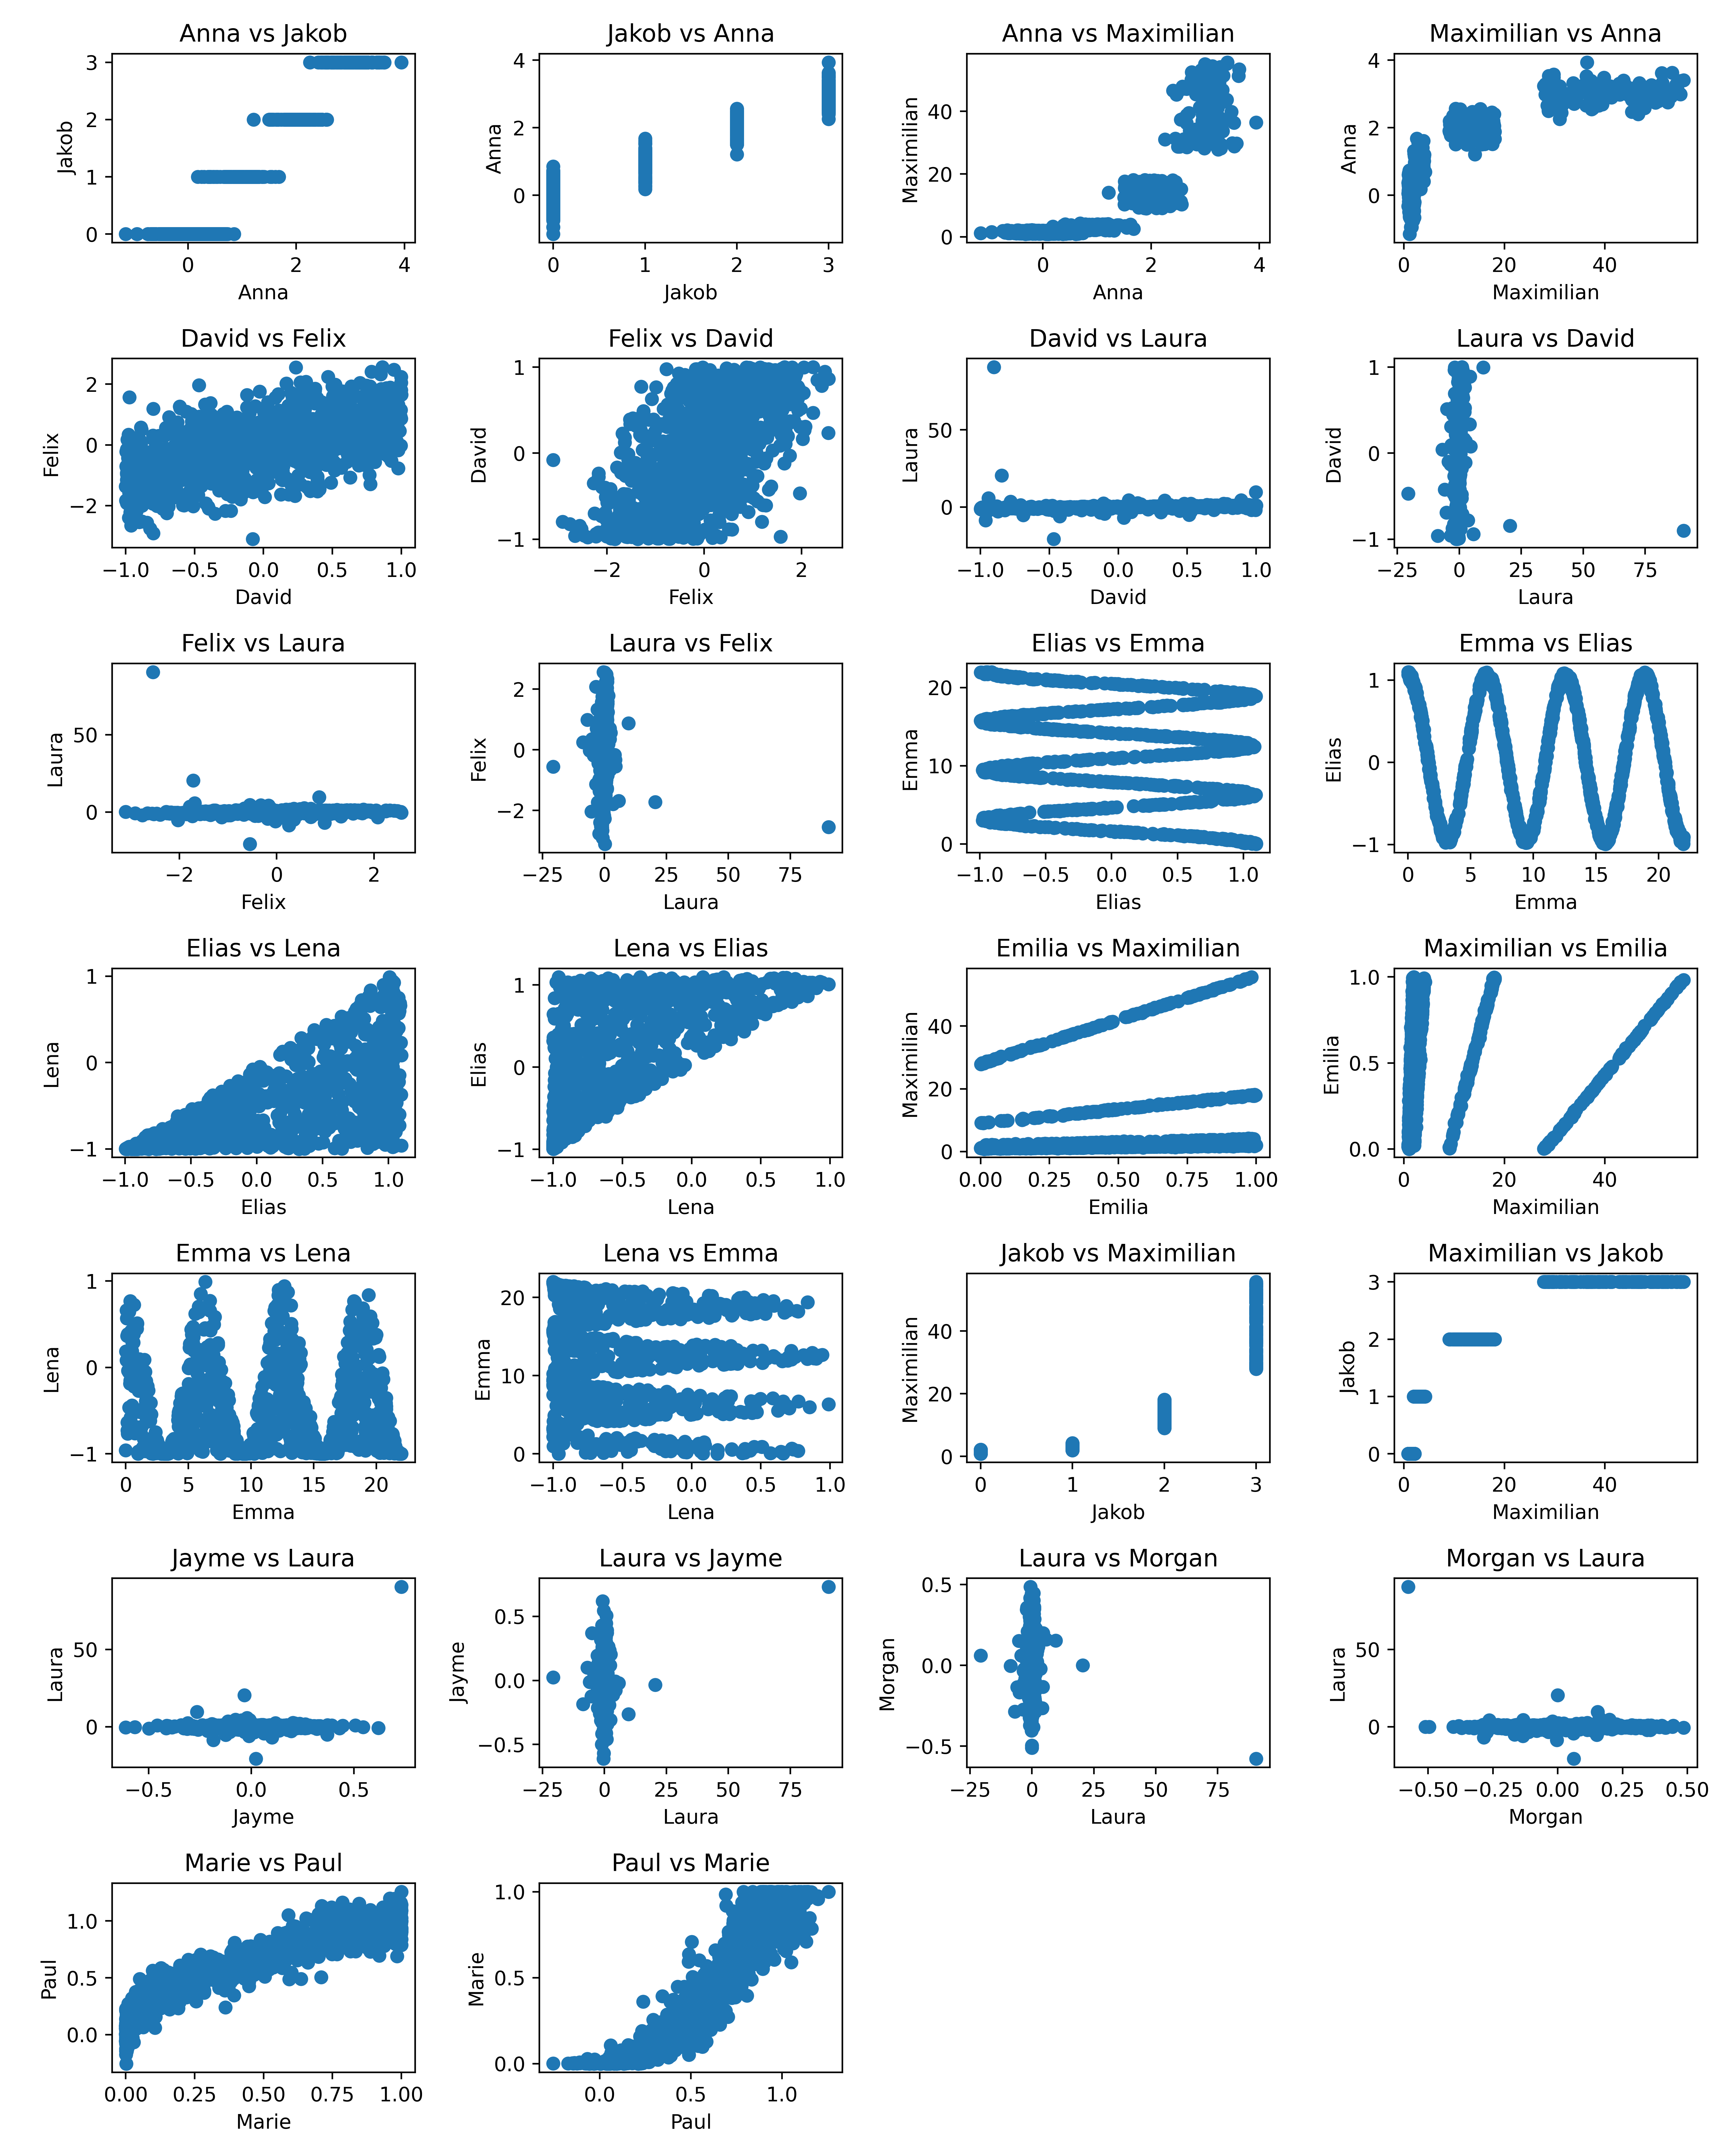
\includegraphics[width=1.1 \textwidth]{figs/best_corr_pairs_adjusted.png}
    \caption{Task 2 -- scatter plots of variables with absolute correlation (coefficient) higher than 0.5 }
    \label{fig:best_pairs}
\end{adjustwidth}
\end{figure}

\begin{figure}
\begin{adjustwidth}{-0.87cm}{}
    \centering
    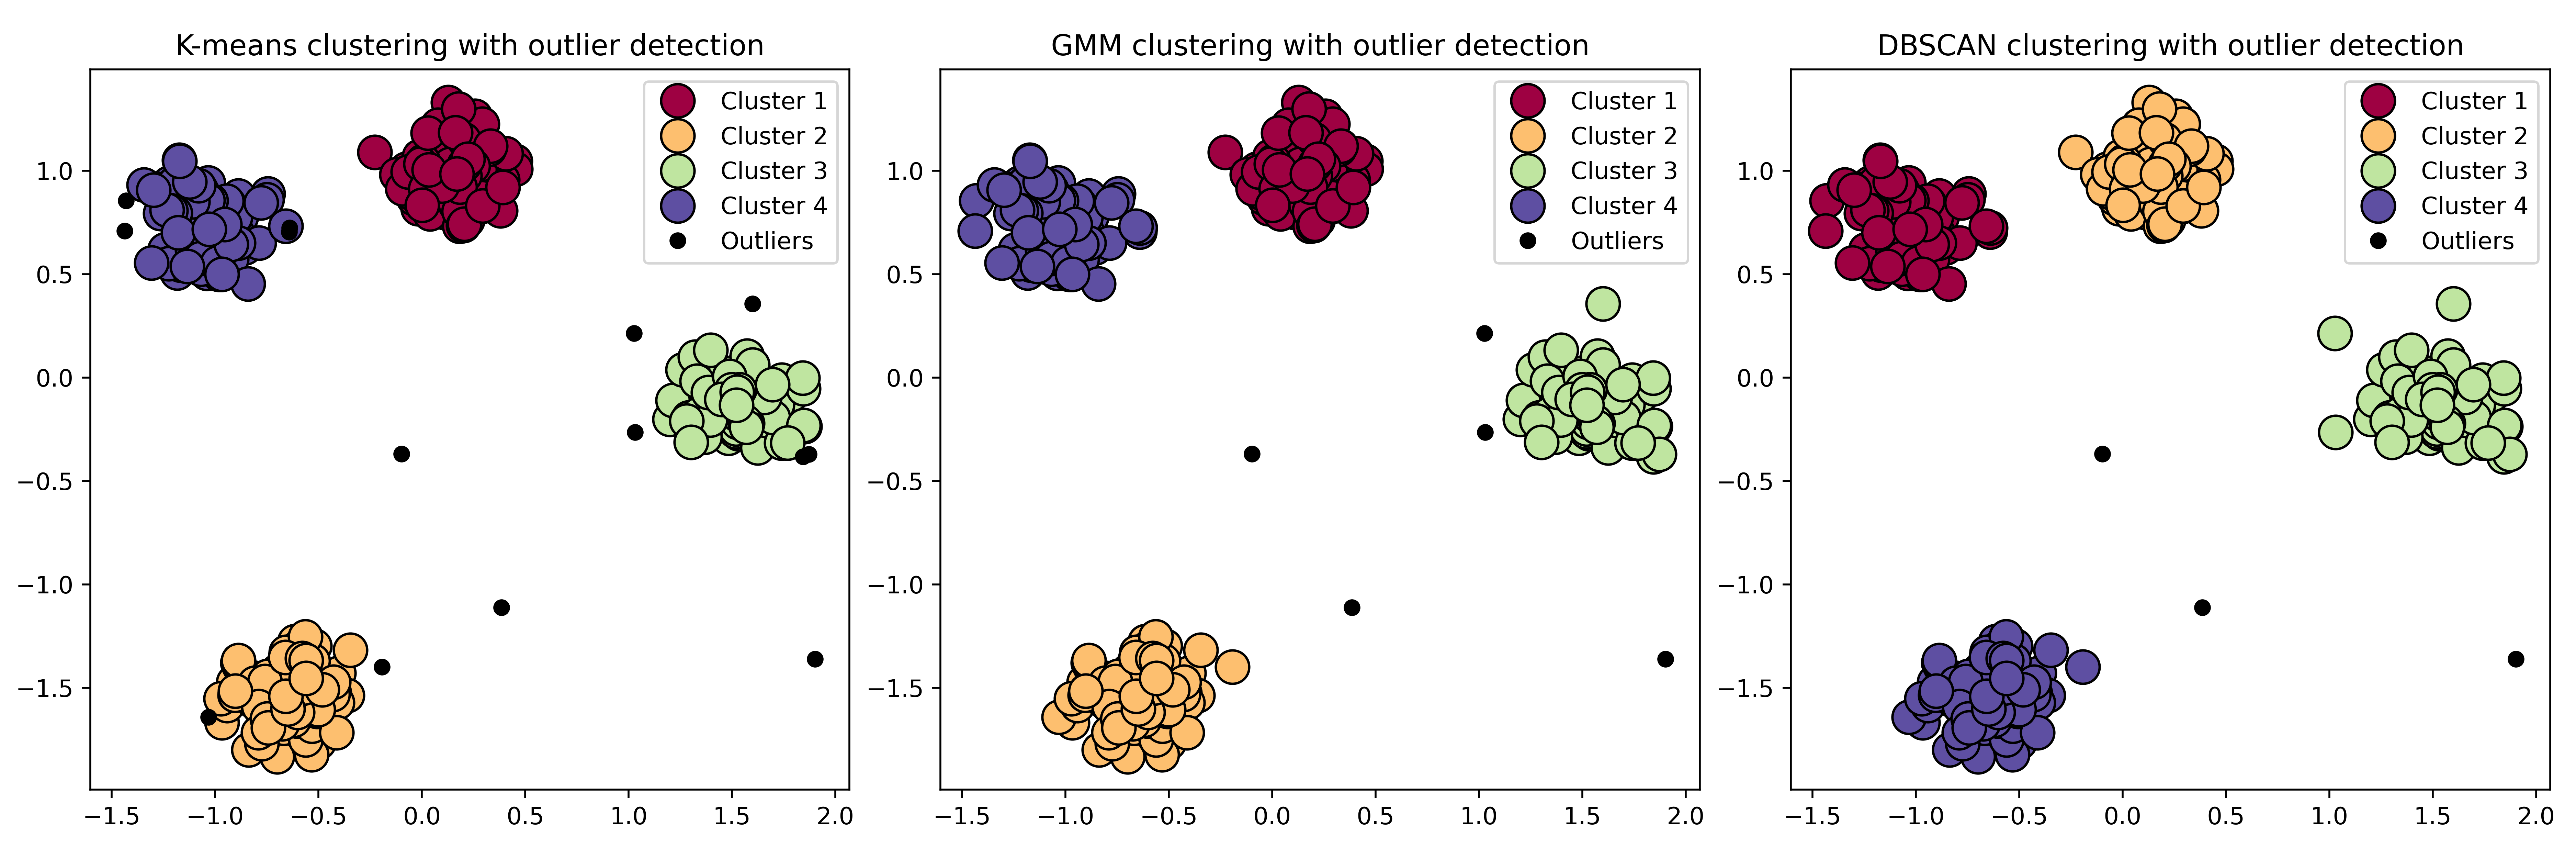
\includegraphics[width=1.1 \textwidth]{figs/outliers.png}
    \caption{Task 3 -- comparison of different methods used for clustering and outlier detection}
    \label{fig:outliers}
\end{adjustwidth}
\end{figure}

\begin{figure}
    \centering
    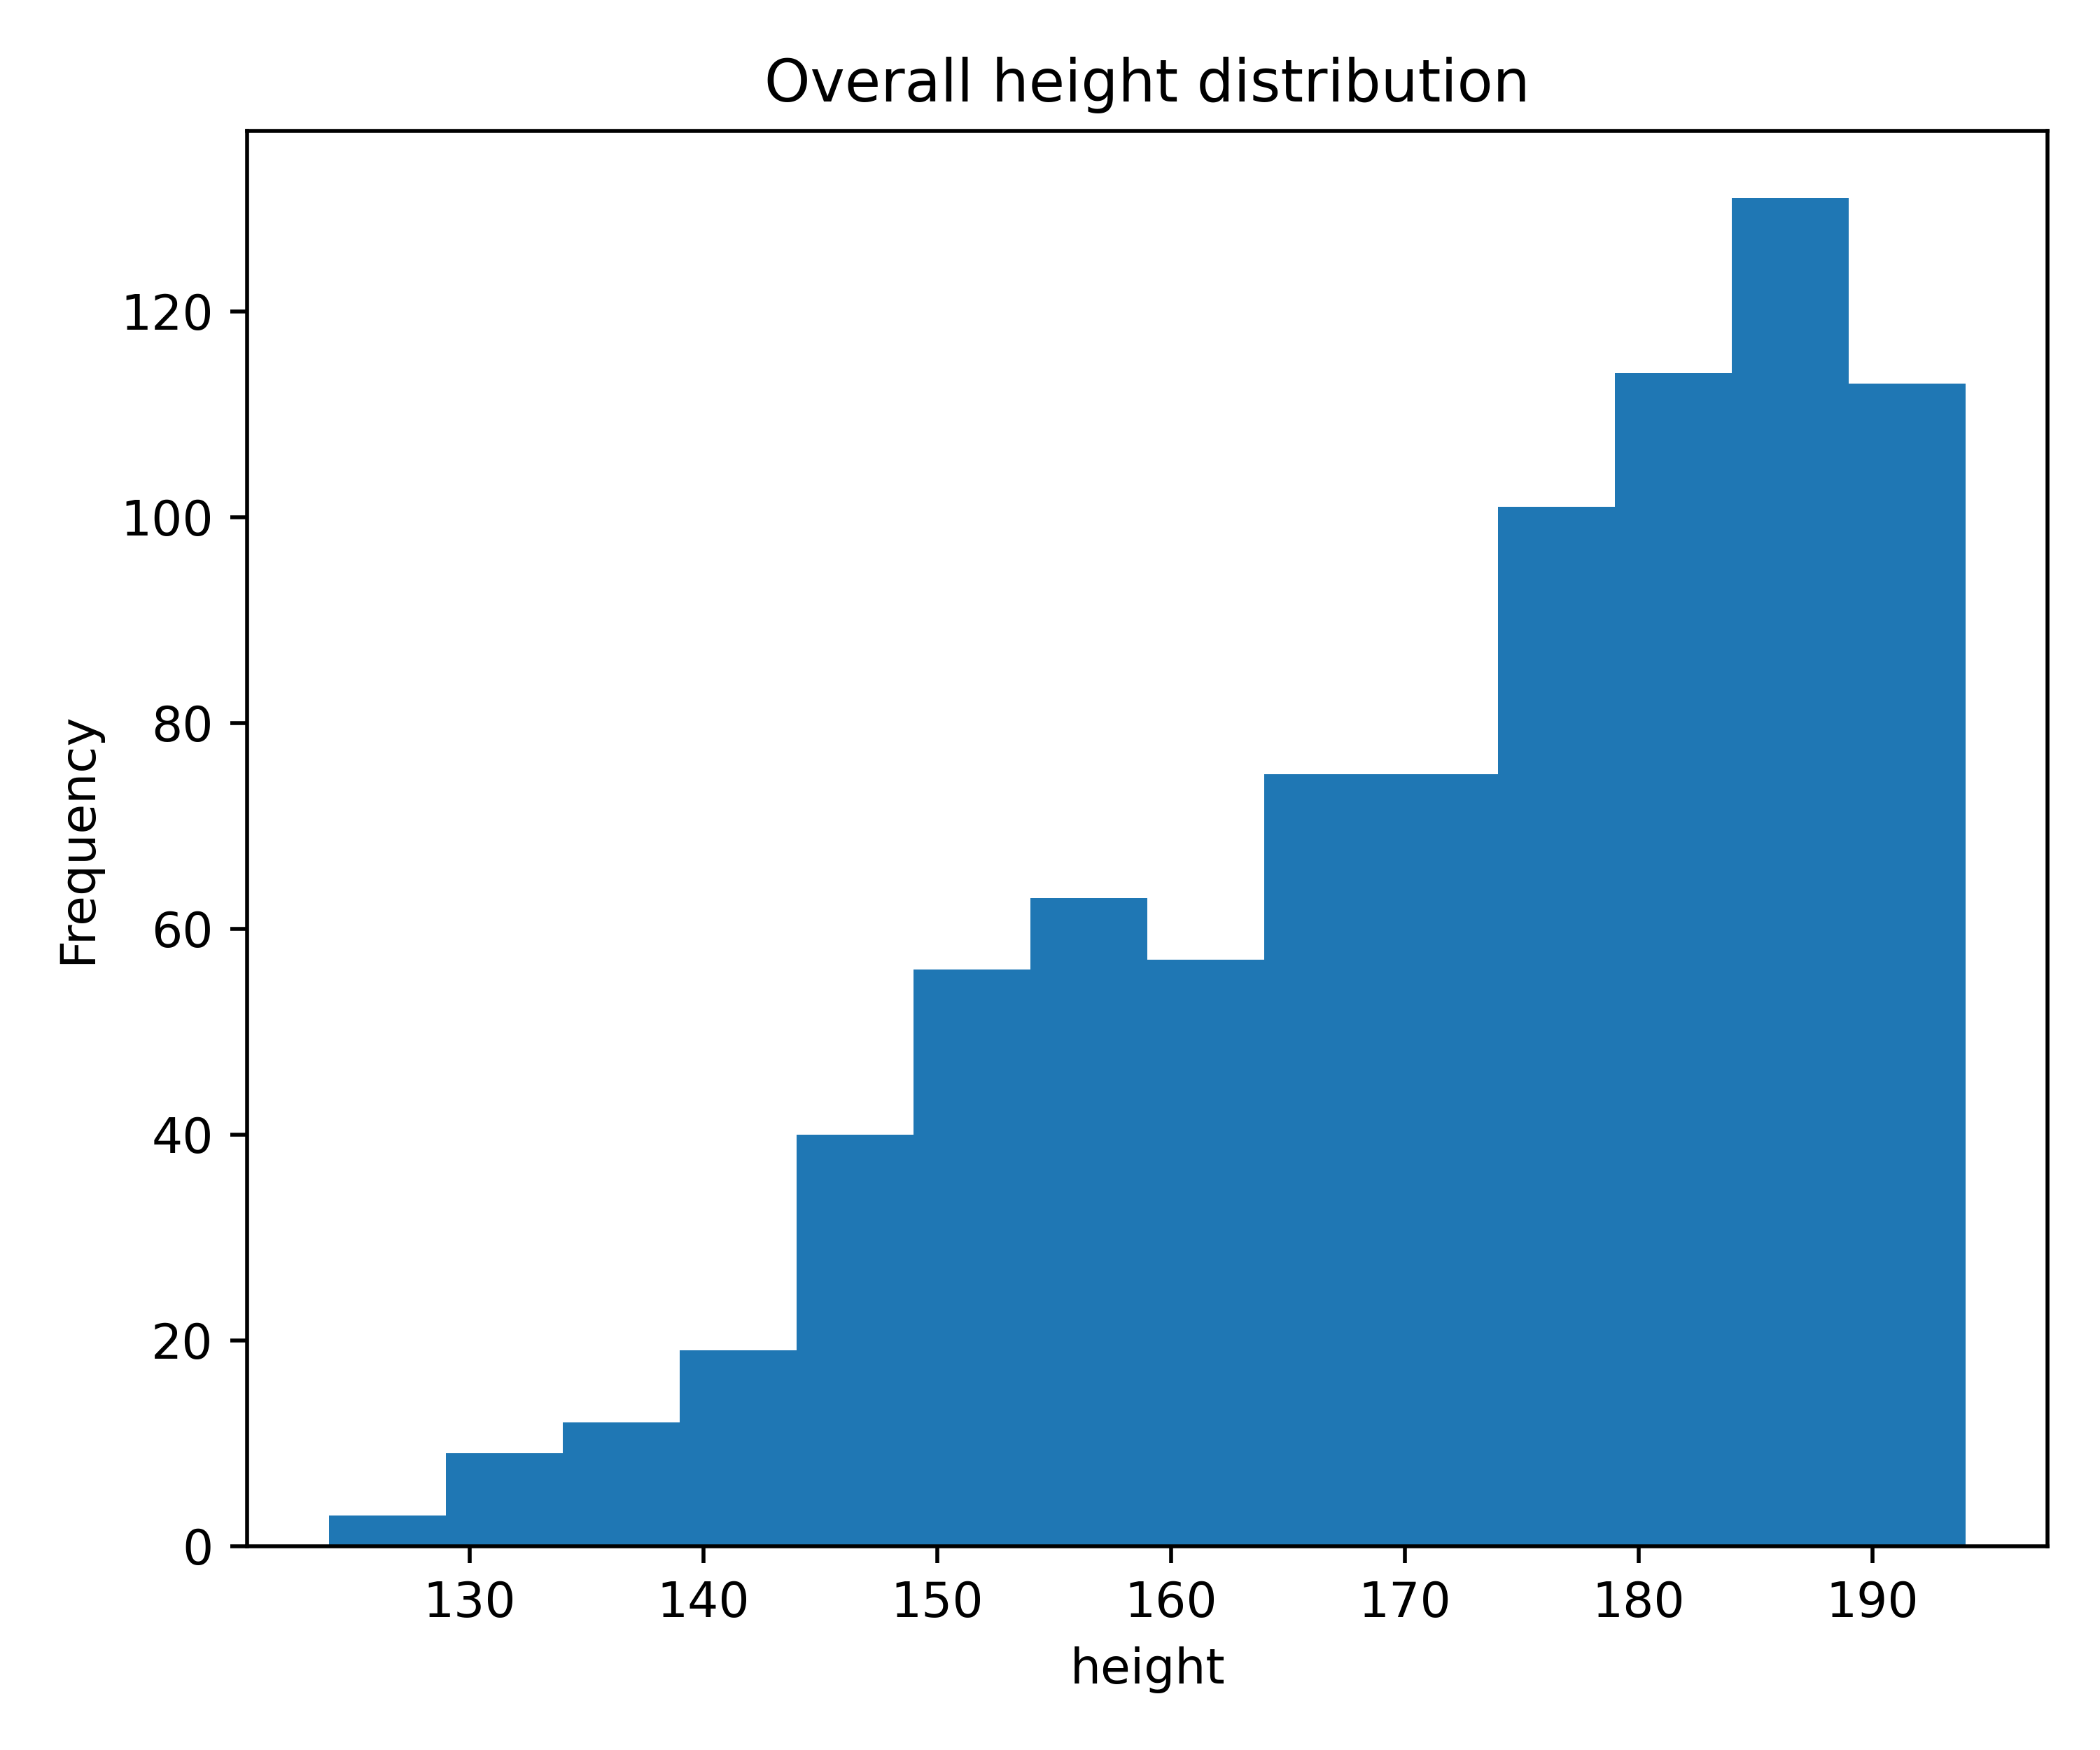
\includegraphics[width=0.5 \textwidth]{figs/height_distribution.png}
    \caption{Task 4 -- overall height distribution}
    \label{fig:height_dis}
\end{figure}

\begin{figure}
\begin{adjustwidth}{-0.87cm}{}
    \centering
    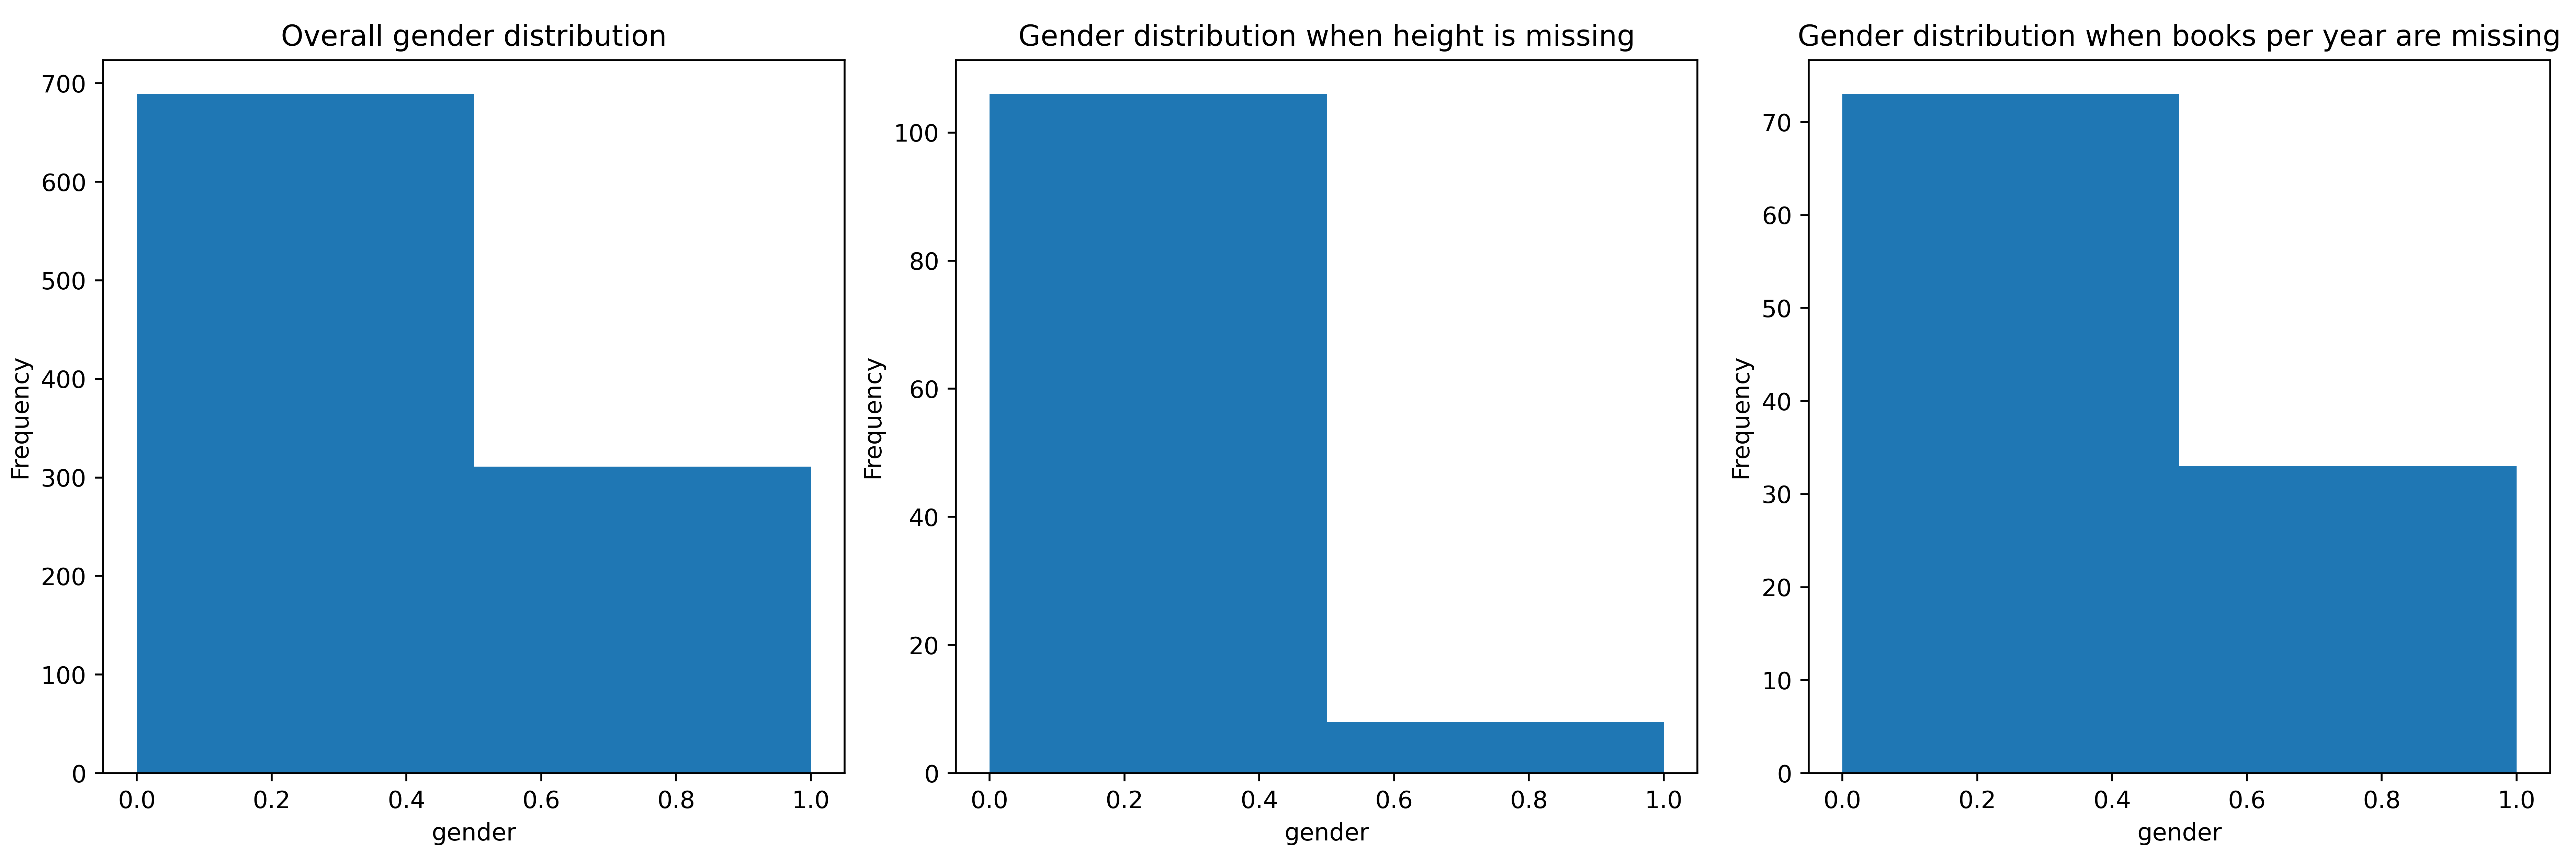
\includegraphics[width=1.1 \textwidth]{figs/gender_distribution.png}
    \caption{Task 4 -- comparison of gender distributions}
    \label{fig:gender_dis}
\end{adjustwidth}
\end{figure}

\begin{figure}
\begin{adjustwidth}{-0.87cm}{}
    \centering
    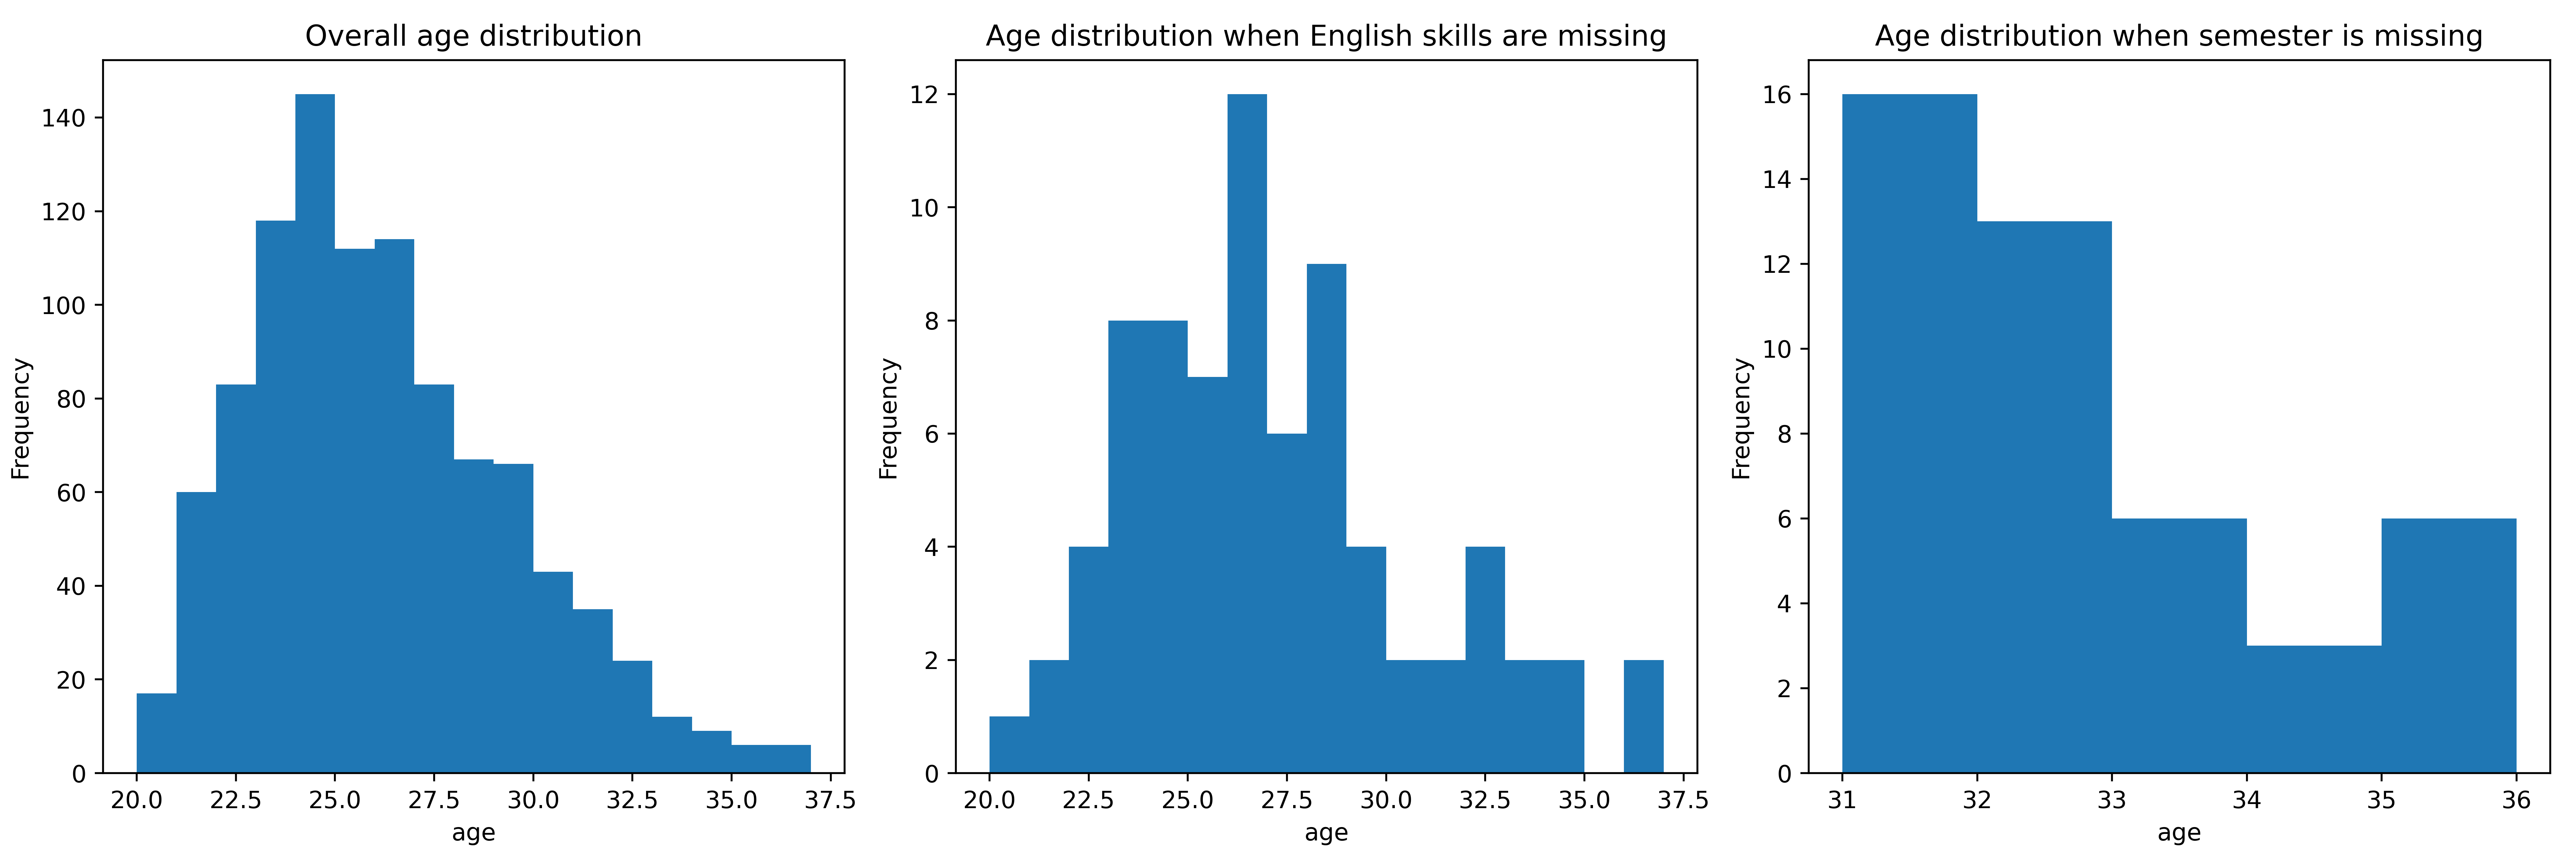
\includegraphics[width=1.1 \textwidth]{figs/age_distribution.png}
    \caption{Task 4 -- comparison of age distributions}
    \label{fig:age_distrib}
\end{adjustwidth}
\end{figure}

\end{document}
